% Copyright (C) 2014-2017 by Thomas Auzinger <thomas@auzinger.name>

\documentclass[draft,final]{vutinfth} % Remove option 'final' to obtain debug information.

% Load packages to allow in- and output of non-ASCII characters.
\usepackage{lmodern}        % Use an extension of the original Computer Modern font to minimize the use of bitmapped letters.
\usepackage[T1]{fontenc}    % Determines font encoding of the output. Font packages have to be included before this line.
\usepackage[utf8]{inputenc} % Determines encoding of the input. All input files have to use UTF8 encoding.

% Extended LaTeX functionality is enables by including packages with \usepackage{...}.
\usepackage{amsmath}    % Extended typesetting of mathematical expression.
\usepackage{amssymb}    % Provides a multitude of mathematical symbols.
\usepackage{mathtools}  % Further extensions of mathematical typesetting.
\usepackage{microtype}  % Small-scale typographic enhancements.
\usepackage[inline]{enumitem} % User control over the layout of lists (itemize, enumerate, description).
\usepackage{multirow}   % Allows table elements to span several rows.
\usepackage{booktabs}   % Improves the typesettings of tables.
\usepackage{subcaption} % Allows the use of subfigures and enables their referencing.
\usepackage[ruled,linesnumbered,algochapter]{algorithm2e} % Enables the writing of pseudo code.
\usepackage[usenames,dvipsnames,table]{xcolor} % Allows the definition and use of colors. This package has to be included before tikz.
\usepackage{nag}       % Issues warnings when best practices in writing LaTeX documents are violated.
\usepackage{todonotes} % Provides tooltip-like todo notes.
\usepackage{hyperref}  % Enables cross linking in the electronic document version. This package has to be included second to last.
\usepackage[acronym,toc]{glossaries} % Enables the generation of glossaries and lists fo acronyms. This package has to be included last.

% Define convenience functions to use the author name and the thesis title in the PDF document properties.
\newcommand{\authorname}{Rebeka Koszticsak} % The author name without titles.
\newcommand{\thesistitle}{Enhancement of Footwear Impressions} % The title of the thesis. The English version should be used, if it exists.

% Set PDF document properties
\hypersetup{
    pdfpagelayout   = TwoPageRight,           % How the document is shown in PDF viewers (optional).
    linkbordercolor = {Melon},                % The color of the borders of boxes around crosslinks (optional).
    pdfauthor       = {\authorname},          % The author's name in the document properties (optional).
    pdftitle        = {\thesistitle},         % The document's title in the document properties (optional).
    pdfsubject      = {Subject},              % The document's subject in the document properties (optional).
    pdfkeywords     = {a, list, of, keywords} % The document's keywords in the document properties (optional).
}

\setpnumwidth{2.5em}        % Avoid overfull hboxes in the table of contents (see memoir manual).
\setsecnumdepth{subsection} % Enumerate subsections.

\nonzeroparskip             % Create space between paragraphs (optional).
\setlength{\parindent}{0pt} % Remove paragraph identation (optional).

\makeindex      % Use an optional index.
\makeglossaries % Use an optional glossary.
%\glstocfalse   % Remove the glossaries from the table of contents.

% Set persons with 4 arguments:
%  {title before name}{name}{title after name}{gender}
%  where both titles are optional (i.e. can be given as empty brackets {}).
\setauthor{}{\authorname}{Bsc}{male}
\setadvisor{Ao.Univ.Prof. Dipl.-Ing. Dr.techn.}{Robert  Sablatnig}{}{male}

% For bachelor and master theses:
\setfirstassistant{Proj.-Ass. Dipl.-Ing.}{Manuel  Keglevic}{}{male}
%\setsecondassistant{Pretitle}{Forename Surname}{Posttitle}{male}
%\setthirdassistant{Pretitle}{Forename Surname}{Posttitle}{male}

% For dissertations:
%\setfirstreviewer{Pretitle}{Forename Surname}{Posttitle}{male}
%\setsecondreviewer{Pretitle}{Forename Surname}{Posttitle}{male}

% For dissertations at the PhD School and optionally for dissertations:
%\setsecondadvisor{Pretitle}{Forename Surname}{Posttitle}{male} % Comment to remove.

% Required data.
\setaddress{Address}
\setregnumber{01325492}
\setdate{04}{01}{2020} % Set date with 3 arguments: {day}{month}{year}.
\settitle{\thesistitle}{Enhancement of Footwear Impressions} % Sets English and German version of the title (both can be English or German). If your title contains commas, enclose it with additional curvy brackets (i.e., {{your title}}) or define it as a macro as done with \thesistitle.
%\setsubtitle{Optional Subtitle of the Thesis}{Optionaler Untertitel der Arbeit} % Sets English and German version of the subtitle (both can be English or German).

% Select the thesis type: bachelor / master / doctor / phd-school.
% Bachelor:
%\setthesis{bachelor}
%
% Master:
\setthesis{master}
\setmasterdegree{dipl.} % dipl. / rer.nat. / rer.soc.oec. / master
%
% Doctor:
%\setthesis{doctor}
%\setdoctordegree{rer.soc.oec.}% rer.nat. / techn. / rer.soc.oec.
%
% Doctor at the PhD School
%\setthesis{phd-school} % Deactivate non-English title pages (see below)

% For bachelor and master:
\setcurriculum{Visual Computing}{Visual Computing} % Sets the English and German name of the curriculum.

% For dissertations at the PhD School:
%\setfirstreviewerdata{Affiliation, Country}
%\setsecondreviewerdata{Affiliation, Country}


\begin{document}

\frontmatter % Switches to roman numbering.
% The structure of the thesis has to conform to
%  http://www.informatik.tuwien.ac.at/dekanat

\addtitlepage{naustrian} % German title page (not for dissertations at the PhD School).
\addtitlepage{english} % English title page.
\addstatementpage

\begin{danksagung*}
\todo{Ihr Text hier.}
\end{danksagung*}

\begin{acknowledgements*}
\todo{Enter your text here.}
\end{acknowledgements*}

\begin{kurzfassung}
\todo{Ihr Text hier.}
\end{kurzfassung}

\begin{abstract}
\par
Shoeprint images are one of the most commonly secured evidences on crimescenes.
Even though automatic shoeprint processing is a highly researched topic, the final identifacion is usually done by human forensic experts.
The two main steps of shoeprint identification are enhancement and matching. 
\par
In this thesis the possibilities for enhancement of shoeprint samples from a real-life dataset are investigated.
The main challange of this task is to correctly filter the pattern regardless the versitile, possibly heavily structured and clutterd noise on the samples.
Two approaches are examined, pattern enhancement and noise suppression.
Among fully automated methods, a semi-automated technique is also tested, where user input is required for noise separation.
\par
The main goal of this work is to find a universal approach which is able to filter and enhance the shoeprint data despite the presence of noise and the possible low image quality.
Based on the experiences acquired while investigating the possible techniques a new noise-supression pipeline for shoeprint images is introduced.
The noisy pixels are identified based on the Fourier-Mellin features of their multi-sized neighborhood.
In the same time a model is built about the average appearance of noise, to eliminate that structure from the foreground as well.
Additionally a gradient based line detector is also applied and the edge structures of the shoeprint are clustered to distinguish between pattern and noise edges.
The experimental results show that the processed images are clearer, the pattern is sharper whereas the noise is either completely eliminated in the background or suppressed in the foreground.
Furthermore based on the results of three differenet basic image descriptor features, the enhanced shoeprints have higher matching rate to their ground-thruth samples than the original images.


\end{abstract}

% Select the language of the thesis, e.g., english or naustrian.
\selectlanguage{english}

% Add a table of contents (toc).
\tableofcontents % Starred version, i.e., \tableofcontents*, removes the self-entry.

% Switch to arabic numbering and start the enumeration of chapters in the table of content.
\mainmatter

\chapter{Introduction}

\par
Shoeprints found on crimescenes can be important hints or evidences in a criminal investigation \cite{kong2014novel}.
Event though on one thrid \cite{alexandre1996computerized} of crimescenes usable shoepatterns can be secured, there is no fully automatized algorithm available yet, which is able to identify and match those prints with the original shoe sole.
Because of that human power is needed \cite{wang2014automatic} to recognize and analyze the found patterns.
The work of forensic experts is not only time consuming and expensive, there is no guarantee about the objectivness of the final outcome\cite{gueham2008automatic}, furthermore the stages of the human matching process are unclear and not necessarily reproducible.
\par
There is an excessive amount of research already done \cite{rida2019forensic} in order to help or repleace the work of forensic experst.
There is however no algorithm published yet, which can be relaiably used in varying conditions and sample quality.
One reason for that are the already mentioned versitile conditions, the features and properties of the pattern on the shoe, like age, material, etc., the characteristics of the ground where the shoeprint is left and enviromental conditions like for example the weather highly influence the overall quality of the acquired sample.
Those high amount of factors result in changing appearance of the prints of the same shoe causing high intra class variance while clustering.
Additionally there is a lack of universal, wide ranged database \cite{rida2019forensic} which correctly depicts the common scenarios occuring on real-life crime scenes.
\par
In 2014 a new database, called FID-300 \cite{kortylewski2014unsupervised} was released which aims to solve the database problem described above.
It contains over 1000 reference shoeprint patterns acquired in a laboratory.
Moreover the database introduces 300 new shoeprint samples collected by the police providing an insight on images forensic experts are working on the daily basis.

\section{Problem Definition}
\par
There are two main stages of automatic shoeprint identification, filtering, where the shoeprint pattern is separated from background and enhanced as well, and matching where the corresponding shoe is determined.
Instead of automatizing the entire shoeprint recogition pipeline this work only focuses on the possible ways of icreasing the sample quality.
Because of the mentioned absence of general, appropiate database it is difficult to compare the already available methods.
Furthermore it is also challanging to estimate which one is applicable in a real-life scenario.
In this thesis multiple possible enhancing techniques are developed and tested in order to find a method which is able to cope with samples taken from real crime scenes.
\par
For evaluation and testing the FID-300 database is used.
The dataset contains both in a laboratory acquired (synthetic) as well as on a crime secured (real) shoeprint patterns.
Additionally there is the Ground Thruth available which real sample which synthetic sample belongs to.
The goal of this work is to define an image processing pipeline which is able to correctly identify and enhance the shoepatterns and eliminate or suppress the noise on the pattern samples regardless the quality of the image.
A secondary objective is to gain an overview about the algorithms already published, and make an estimation which methods are applicable in real-life scenarios based on their performance on the FID-300 database.

\section{Challanges}
\par
There are two main obsticles in the topic of shoeprint enhancement and in automatic shoeprint matching in general, the versitile image quality and appearance and the lack of universal and wide database.
The shoeprint patterns are varying, there are approaches available which build models for given structures of the shoeprint \cite{tang2010footwear}, \cite{alizadeh2017automatic}, but no detailed, uniform representation for the entire shoeprint is possible.
Moreover there is a high inference of noise from multiple sources.
The ground where the shouprint is found is considered as noise expect in the rear case when it is left on a non changing, even surface.
The produced print of the same shoepattern varys on different type of surface.
Additionally the roughness and unevenness of a given type of surface also distorts the original pattern.
Furthermore other objects on the ground, on or behind the left shoeprint can cover or distort the original pattern, or they can prevent to leave a print on their area completely.
Besides that the pattern on the original shoe can also be distorted or modified compared to the new version.
Distortions caused by usage are valuable information about the owner, on the other hand they make it more difficult to match the pattern with their unused pairs.
Additional objects between the structures of the shoeprint also alter the original appearance.
Lastly, there are multiple shoeprint securing methods producing different results for the same print \cite{katireddy2017novel}. 
The shoeprint lifting technique used depends on the properties of the ground. 
Those two factors, the securing method and the floor, also determine if the positive or the negative, the actual pattern or the space between the shoeprint structures, image is captured.
\par
The non-existing universal database causes that two published methods are difficult to compare based on their results since they are using different testing images.
The used dataset is not necessarily published \cite{katireddy2017novel}, \cite{dardi2009texture} making it impossible to reproduce the reulst in those cases.
Additionally the handcrafted databases can be biased, and allow such restrictions and modifications which do not correlate with real-life scenarios \cite{rida2019forensic}.
The used samples are either synthetically generated and computationally distorted \cite{de2005automated}, \cite{gueham2008automatic} or exlude low quality and noisy images \cite{dardi2009texture}, \cite{tang2010footwear}.
Because of that it is difficult to compare their performance and to estimate which one of the published approaches are applicable on the FID-300 database.
Furthermore it is challanging to plan a new algorithm based on the published results because their lack of a uniform baseline.

\section{Contribution}
\par
In this thesis the possible ways of enhancing a shoeprint images are discussed.
Because of the known issues on database multiple approaches are implemented, discussed and evaluated.
The two ways to increase the quality of a given shoeprint sample is to enhance the pattern regardless of the noise and to supress or eliminate the noise without losing any of pattern information.
Along fully-automated methods semi-automated possibilities are also considered.
Three different approaches are introduced and examined for their performance on real-life image samples.
\par
Finally a new semi-autoamted framework is given which is evaluated on the FID-300 database.
In the first step user ipnut about the noise is required.
The input is separated into tiles, and the subparts are compared based on the Fourier-Mellin features to the region of the use input.
In that way the background is separated from the foreground and the average appearance of the image is calculated.
Since noise appears on the pattern as well, the distorted parts are corrected based on the calculated noise model.
After that gradient based line detection is perfromed and the results are separated into clusters where pattern and noise classes are defined and candidates of the latter are eliminated.
The final image is thresholded to create a binary image, where the shoeprint is clearly visible and recognizable whereas the clutter is supressed on the pattern and eliminated in the background of the image.
Throughout the whole processing pipeline morphological opeartions and small structure elimination is applyed multiple times.
First when a mask for background is built, and also in the end of the pipeline to eliminate small inconsistencies on the pattern.
Experimental results show, that the enhanced images are clearer, the background is successfully eliminated and the shoeprint pattern is less noisy than on the original images.
Figure \ref{fig:example} shows an example sample from the FID-300 database \ref{fig:intro:orig} and the enhanced images \ref{fig:intro:enhanced} with the proposed algorithm.
Moreover the  matching of the sample and the enhanced images with their in a laboratory lifted pair according to basic image features such as SIFT and SURF indicate that the improved images have a better matching rate than its original version.


\begin{figure}[h]
  \centering
  \begin{subfigure}[b]{0.45\columnwidth}
    \centering
    \includegraphics[width=\textwidth]{1/00182.jpg}
    \subcaption{Example image from the FID-300 database}
    \label{fig:intro:orig}
  \end{subfigure}
  \begin{subfigure}[b]{0.45\columnwidth}
    \centering
    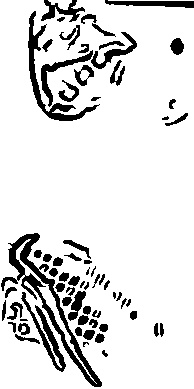
\includegraphics[width=\textwidth]{1/00182_filtered.jpg}
    \subcaption{Enhanced image}
    \label{fig:intro:enhanced}
  \end{subfigure}
  \caption{Result of the proposed algorithm}
  \label{fig:example}
\end{figure}

\section{Structure of the Work}
\par
To gain an overview about the research already done the followong section, Capter 2, gives a review about the literature. 
Along papers published in the topic of shoeprint identification, matching and enhancement, research of similar domains is presented as well.
Fields of fingerprint processing and tattoo identification is also overviewed for possibilities of using the tecniques in the given problem.
Furthermore natural image enhancement and denoising tecniques are revised as well.
\par
In Chapter 3, 4 and 5 the approaches for enhancement are given and discussed if they are applicable for real-life forensic images.
Chapter 3 presents and evaluates a possible way for pattern enhancement.
Chapter 4 and 5 describes an automated and a semi-automated noise supression pipeline respectively.
In Chapter 5 the new algorithm for enhancing real-life crimescene shoeprint impressions is proposed.
Details on implementation are revealed as well.
\par
In Chapter 6 experimental results are shown and the proposed algorithm is evaluated.
In Chapters 7 and 8 prospective future work is discussed and the final conclusion is given. 

\chapter{Related Work}
\par
In order to find and develop an effective algorithm for shoeprint enhancement an overview about relevant research has to be made first.
Along the evident litrtiture of image enhancement and noise removal a further, related topic discriminative image descriptors are also considered, to gain the best insight possible and to be able to develop an algorithm which is optimized for the rest of the shoeprint identification pipeline.
In this chapter the research on the domain of shoeprint identification is reviewed.
Other than that publications from similar domains such as fingerprint and palmprint detection as well as tattoo identification are described.
The related domains fingerprint identification and tatto recognition have been choosen for review because of their similar goal of edge structure and minimal image structure recognition.
Moreover an overview of techniques from the field of natural image enhancement and description along with general image denoising is also given.
This chapter is separated into four parts, first Image Enhancement techniques are described, after that algorithms developed for Noise Removal specifically are discussed.
In the second half of the chapter proposed methods Image Descriptors and lastly for Featuree Classifications are reviewd

\section{Image Enhancement}
\label{sec:rw:ImageENhancement}

In this section image enhancement tecniques from four specific domains are discussed, these are shoe- and fingerprint identification, tattoo recognition and natural image enhancement.

\section*{Shoeprint Enhnacement}

\par
There is an extensive research done in the field of enhancing shoeprint images.
However, it has to be noticed that the problem definition and the use-case of the different publications varys.
Becuse of the absence of standrad database, the discussed algorithms can be separated into two groups, techniques tested on synthetic samples and on real-life impressions.
Synthetic samples are images scanned in images in a laboratorial enviroment for the purpose of building a dataset for shoeprint identification.
The noise derives from scanning artifacts and computationally added distortions and modification.
Furthermore many algorithms developed for real crime-scene data make restrictions about the input image and exclude noisy and poor quality images.
Figure \ref{fig:rw:database} shows example images from a synthetic \ref{fig:rw:synthetic}, from a restricted \ref{fig:rw:restricted} and high \ref{fig:rw:highFID} and low quality samples \ref{fig:rw:lowFID} from the FID-300 dataset.
In the following discussion it is noticed repeatedly, which kind of dataset the proposed approach was tested on.

\begin{figure}[h]
  \centering
  \begin{subfigure}[b]{0.24\columnwidth}
    \centering
    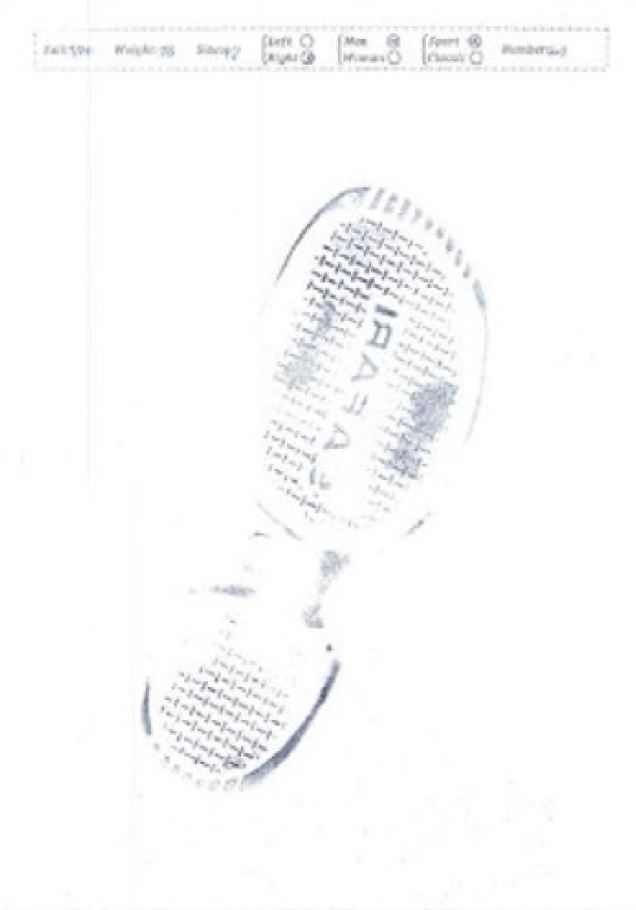
\includegraphics[width=\textwidth]{2/synthetic.jpg}
    \subcaption{Example image from a synthetic dataset}
    \label{fig:rw:synthetic}
  \end{subfigure}
  \begin{subfigure}[b]{0.24\columnwidth}
    \centering
    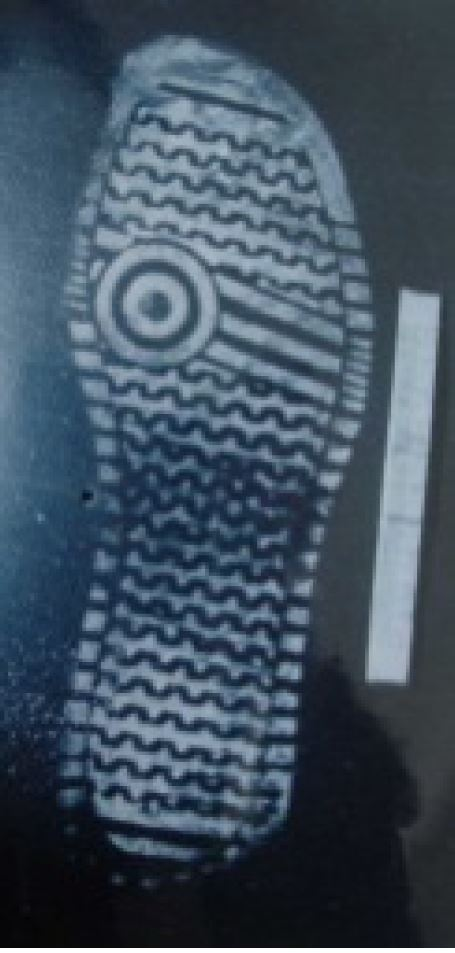
\includegraphics[width=\textwidth]{2/restricted.jpg}
    \subcaption{Example image from a real crimescene dataset exluding low quality images}
    \label{fig:rw:restricted}
  \end{subfigure}
  \begin{subfigure}[b]{0.24\columnwidth}
    \centering
    \includegraphics[width=\textwidth]{2/00025.jpg}
    \subcaption{Example high quality image from the FID-300 database}
    \label{fig:rw:highFID}
  \end{subfigure}
  \begin{subfigure}[b]{0.24\columnwidth}
    \centering
    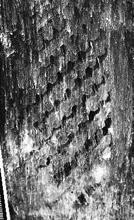
\includegraphics[width=\textwidth]{2/00174.jpg}
    \subcaption{Example low quality image from the FID-300 database}
    \label{fig:rw:lowFID}
  \end{subfigure}
  \caption{Example images of a synthetic \cite{alizadeh2017automatic}, of a restricted \cite{li2014retrieval} and of the FID-300 \cite{kortylewski2014unsupervised} dataset}
  \label{fig:rw:database}
\end{figure}

\par
Morphological Operations, Thresholding and Image Filtering are popular techniques for improve the quality of both kind, realistic and synthetic, of input data.
Morphological operations, especially Opening and Closing, is used in many cases \cite{wang2014automatic}, \cite{kong2014novel}
, \cite{li2014retrieval}, \cite{tang2010footwear}, \cite{wu2019crime}, whereas Wang et al. \cite{wang2014automatic} uses a synthetic dataset, and other than Wu et al. \cite{wu2019crime} the forensic images are restricted to high quality data.
 Wang et al. \cite{wang2014automatic}, Kong et al.  \cite{kong2014novel} and Li et al. \cite{li2014retrieval} use the Morphological Operations to correct inconsistencies after thresholding.
Similar to the previous approaches Wu et al. \cite{wu2019crime} applies the same pipeline on a real forensic dataset.
Tang et al. \cite{tang2010footwear} follow the same principle but instead of thresholding, after Canny edge detection is Opening and Closing used.
\par
To create a binary image and eliminate noise various thresholding techniques are used.
Otsu  \cite{wu2019crime}, \cite{algarni2008novel}, \cite{alizadeh2017automatic}, \cite{kong2014novel} and adaptive thresholding \cite{wang2014automatic}, \cite{li2014retrieval} are the two most popular algorithms.
Algarni et al. \cite{algarni2008novel} and Alizedah et al. \cite{alizadeh2017automatic} along with Wang et al. \cite{wang2014automatic} published their algorithms for synthetic datasets.
Kong et al. \cite{kong2014novel} and Li et al. \cite{li2014retrieval} tested on restricted, whereas Wu et al. \cite{wu2019crime} developed their approach for full real forensic database.
Wang et al. \cite{wang2014automatic} and Wu et al. \cite{wu2019crime} combine thresholding with a grid based approach to calculate exact thresholds for every subarea of the picture.
\par
An other way to eliminate noise is image filtering.
Alizadeh et al. \cite{alizadeh2017automatic} uses a simple Median filter on a synthetic dataset.
Zhang et al. \cite{zhang2005automatic} test on synthetic database as well.
They take advantage on the partial different equations approach.
In this way the edges are preserved while the background is smoothed according to a controlled curvature motion criteria. 
Katireddy et al. \cite{katireddy2017novel} uses Successive Mean Quantization Transfrom (SMQT) \cite{nilsson2013smqt} as an only step to ehnace a real-life database.
Figure \ref{fig:rw:SMQT} shows the output of the SMQT algorithm on an example image.

\begin{figure}[h]
  \centering
  \begin{subfigure}[b]{0.4\columnwidth}
    \centering
    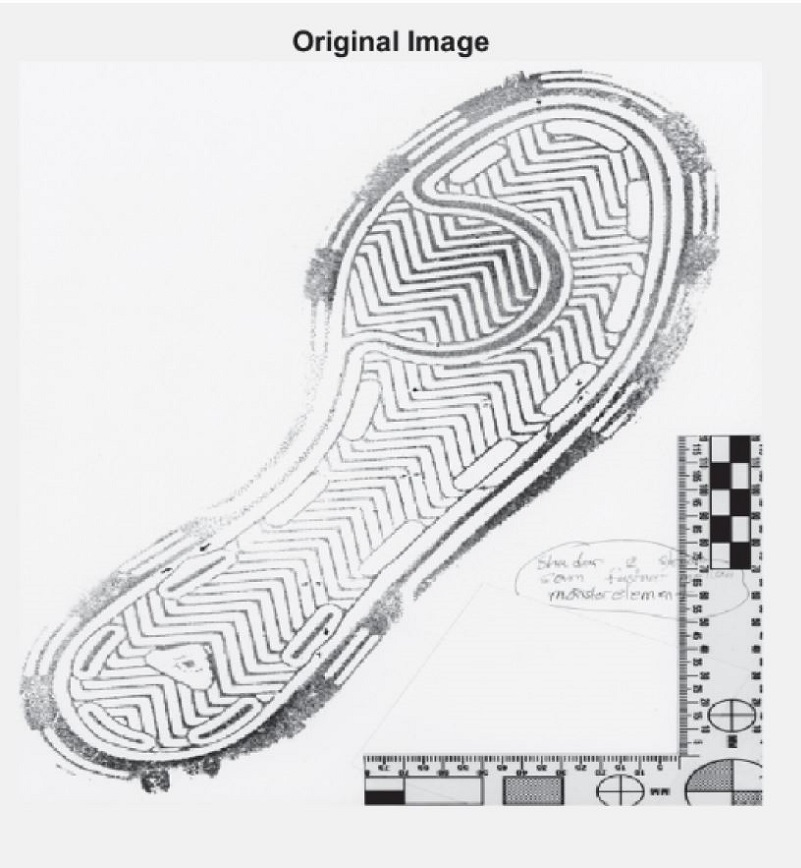
\includegraphics[width=\textwidth]{2/SMQTorig.jpg}
    \subcaption{Example shoeprint impression}
    \label{fig:rw:SMQTin}
  \end{subfigure}
  \begin{subfigure}[b]{0.4\columnwidth}
    \centering
    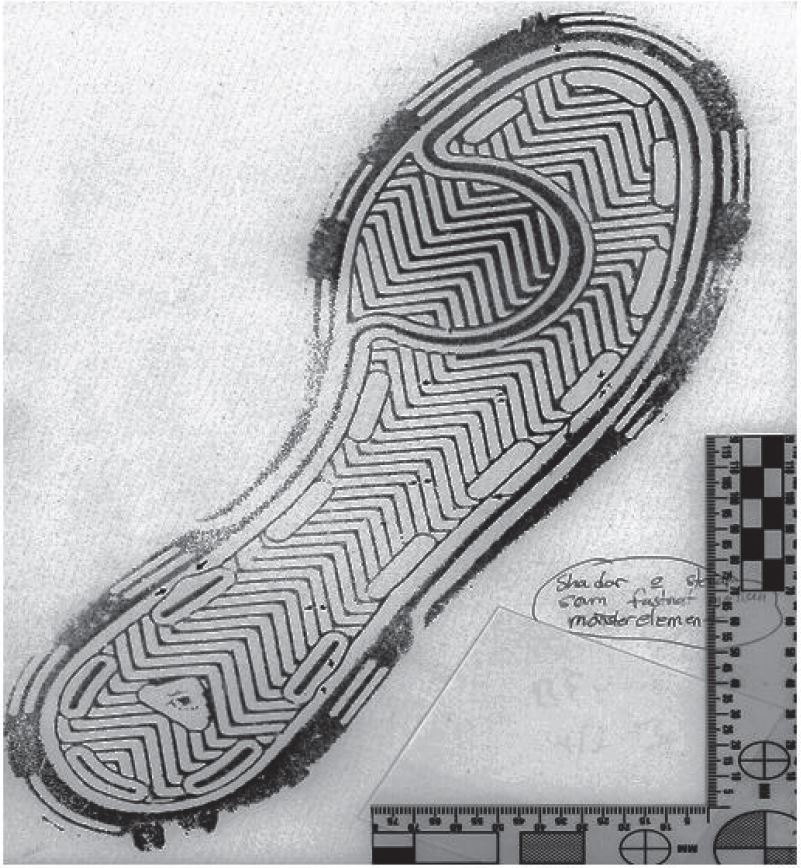
\includegraphics[width=\textwidth]{2/SMQT.jpg}
    \subcaption{Enhanced image with the SMQT algorithm}
    \label{fig:rw:SMQTout}
  \end{subfigure}
  \caption{Example image about the enhancement feature of the SMQT algorithm \cite{katireddy2017novel} }
  \label{fig:rw:SMQT} % \label has to be placed AFTER \caption (or \subcaption) to produce correct cross-references.
\end{figure}

\par
Bandpass operators are also used for noise supression.
The images are converted to the frequency domain where high and low frequencies are eliminated.
Gueham et al. \cite{gueham2007automatic} and Richetelli et al. \cite{richetelli2017classification} utilize this method on a synthetic database.
Li et al. \cite{li2014retrieval} work with a restricted real dataset, where only the lower frequencies are eliminated.
Another frequency based approach was proposed by Katireddy et al. \cite{katireddy2017novel} based on Daubechies wavelets.
After SMQT enhancement the Daubechies wavelets are used to separate the fore- and background and to remove the noise in the latter.

\section*{Fingerprint Enhnacement}

Bandpass and general image filtering is popular in the field of fingerprint enhancement as well.
Zhou et al. \cite{zhou2011adaptive} uses a low- and a highpass filter to eliminate striking frequencies. 
Baig et al. \cite{baig2015enhancement} apply Directional Hilbert transform of a Butterworth andpass to collect the different phase shifts and eliminate the artifacts created by previous thresholding of the input.
Wang et al. \cite{wang2014enhanced} decompose the image into four subbands and process them separately, calculating the noise for every subband respectively.
Li et al. \cite{li2012texture} use Fourier transformation combined with Scale Invariant Feature Transform (SIFT) to enhance the fingerrint images. \todo{reference}
With SIFT the intresting points in the Fourier domain are found and secured, while the image is filtered to suppress noise and other inconsistencies.
Jahan et al. \cite{jahan2017robust} apply Fuzzy filtering followed by thinning.
Fuzzy filter is a local method to preserve the edge information and fine lines structures and supress the noisy background of the input.

\section*{Tattoo Enhnacement}

For tattoo enhancement an algorithm from Han et al. \cite{han2013tattoo} was proposed which combines Gaussian filtering with Hysteresis thresholding. \todo{reference}
Hysteresis thresholding is a neighborhood-aware approach where a pixel is labelled when it is above a given low threshold and simultaneously connected to other pixels meeting a higher thresholding criteria. \todo{reference}
Acton et al. \cite{acton2008matching} propose to use an Active Contour Model to find the boundaries of tattoo images and apply Opening and Closing as well to get rid of small inconsistencies.

\section*{Natural Image Enhnacement}
\par
Along Signal, especially Bandpass, general Image Filtering and Thresholding Histogram and Color Operations are also common for natural image enhancement.
Maini et al. \cite{maini2010comprehensive} published a review about natural image enhancing algorithms and defined two main groups of algorithms, Frequency and Spatial Domain Methods.
First publications utilizing techniques from the first group are discussed, after that the usage of Spatial Domain Methods is reviewed.
\par
Xu et al. \cite{xu2016image} combines Bandpass filtering with adaptive thresholding.
Similar to Wang et al. \cite{wang2014enhanced} the image is separated into four subbands, and the threshold is calculated for every image separately.
Sugamya et al. \cite{sugamya2016image} applies Subband Decomposition with two staged Histogram Equalization.
The histogram of the input is equalized gloablly first, after that it is decomposed into subbands to Equalize the values locally for every four generated subimage.
\par
Median Fiters are used for noise suppression no only in the domain of shoeprint enhancement \cite{alizadeh2017automatic} but also for natural image processing.
Apart from Median Filter Li et al. \cite{li2014rapid} utilize Average and Wiener Filter as well to suppress the occuring noise and to prepare the input for neighborhood based feature extraction.
Feng et al. \cite{feng2011bag} proposed a Bag-of-Words algorithm based on the Gabor wavelets of the input. 
For preprocessing the Watershed Transform is used.
\par
Histogram Operations can be combined with not only Bandpass filtering as Sugamya et al. \cite{sugamya2016image} do but also with Thresholding as proposed by Yao et al. \cite{yao2016image}.
Their aprroach separates the histogram of the input into two parts according to Otsu\'s method.
After that the histogram is equalized of the generated subimages.
Figure \ref{fig:rw:BHNMT} shows the results of algorithm on an example image.

\begin{figure}[h]
  \centering
  \begin{subfigure}[b]{0.4\columnwidth}
    \centering
    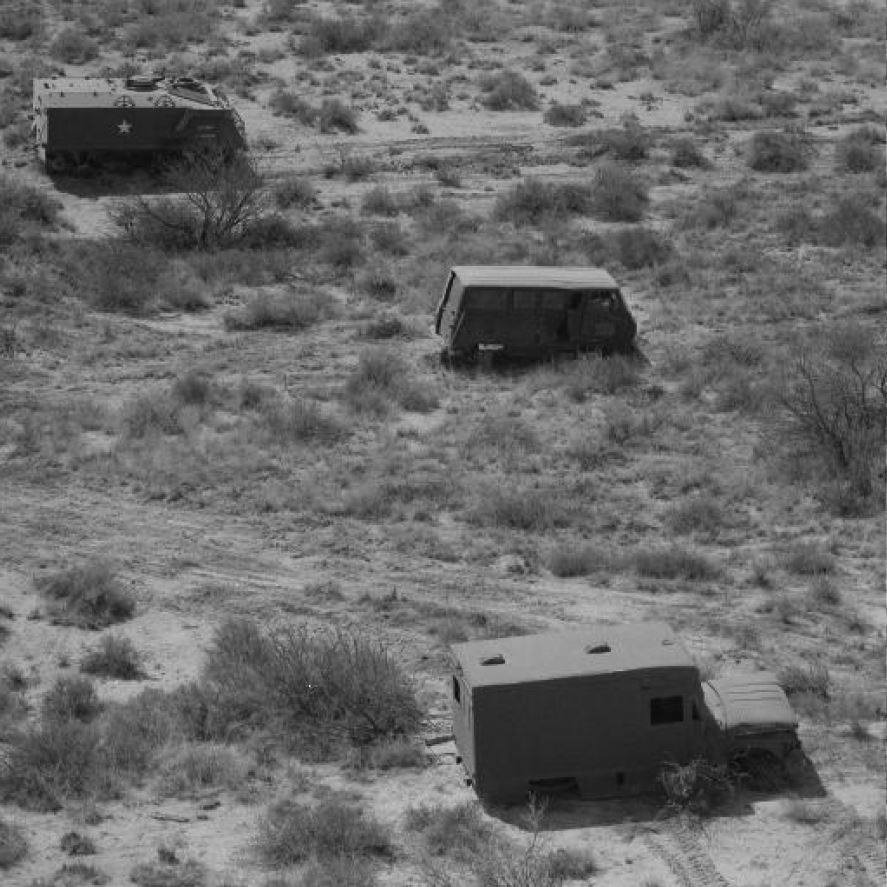
\includegraphics[width=\textwidth]{2/BHNMTorig.jpg}
    \subcaption{Example low-contrast image}
    \label{fig:rw:BHNMTin}
  \end{subfigure}
  \begin{subfigure}[b]{0.4\columnwidth}
    \centering
    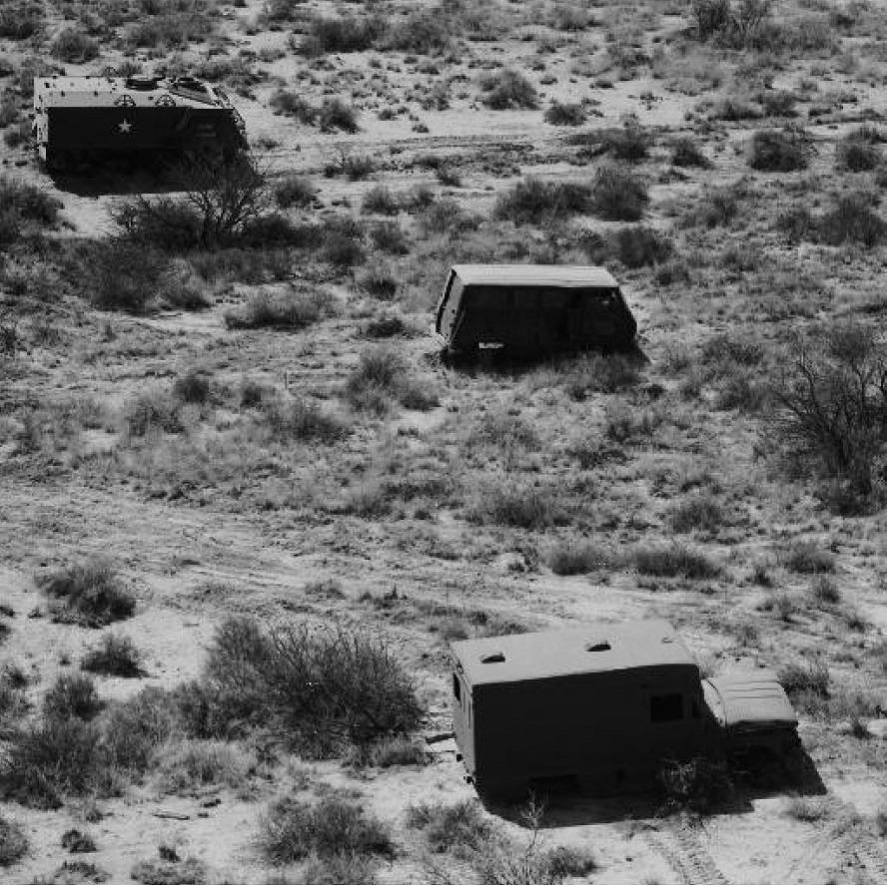
\includegraphics[width=\textwidth]{2/BHNMT.jpg}
    \subcaption{Enhanced image with the histogram thresholding algorithm}
    \label{fig:rw:BHNMTout}
  \end{subfigure}
  \caption{Example image  \cite{yao2016image} about the enhancement feature of the algorithm proposed by Yao et al. \cite{yao2016image} }
  \label{fig:rw:BHNMT} % \label has to be placed AFTER \caption (or \subcaption) to produce correct cross-references.
\end{figure}

\par
Color processing techniques are widespresd in he topic of natural image enhancement.
It can be used for image dehazing, so for low contrast images, \cite{singh2018dehazing} and also for classical noise removal \cite{ren2018joint}, \cite{zhang2016simultaneous}. 
Bhairannawar et al. \cite{bhairannawar2017color} switch from RGB to HSV and use Laplace filter to detect regions with intensity changes. 
During processing the H chanel is not modified to prevent color distortion artifacts.
Althoug color processing is a well researched field with many promissing solutions, no wider overview is given in this thesis.
There are shoeprint impression datasets with colored samples, FID-300 provides grayscale images thus no color processing approach can be used in this specific case. 

\section{Noise Removal}

Noise Removal methods are based on estimating the original image, and based on that eliminating the deviating features of the data.
One way is denoising through gradient histogram preservation \cite{zuo2013texture}.
The distribution of gradients is estimated on the original image, and the noisy image is adjusted to the calculated values.
An alternative way is to decompose a single image and based on the clear parts the noisy regions are approximated.
Huang et al. \cite{huang2013self} propose a self-learning algorithm, which only consideres the high frequency parts of the decomposed image.
There were several approaches published, where the images is separated is separated spatially instead of in the frequncy domain.
\cite{xu2015patch}, \cite{talebi2013global}, \cite{chatterjee2011patch} and \cite{guo2015efficient} are tecniques based on the idea of non-local means, where the image is subsampled into tiles and the pixels are set to the mean of regions belongng to the same cluster.
The main difference between the previous algorithms is how they classify the image subregions into different classes.
Taleby et al. \cite{talebi2013global} uses an iterative shrinkage strategy. 
Chatterjee et al.  \cite{chatterjee2011patch} groups the geometrically similar regions and estimate the noise for every class separately with a Wiener Filter.
Whereas Guo et al. \cite{guo2015efficient} utilize Block Matching to determine the cluster memberships. 
Additionally the spatial location is also considered while calculating the mean value in a given class.
The members are weighted according to the distance to the current region.

\section{Image Description}

Similar to the previous Image Enhancement section \ref{sec:rw:ImageENhancement} this part is also subdivided into four domains offering solutions for the same problem in different domains.
In this section the published image features are described which are proposed to be the most discriminative for their field.
Similar topics are reviewd to gain insight about the most powerful descriptors and consider to port them into the domain of this thesis.
Shoeprint descriptors are described first, after that fingerprint features are discussed.
Following that an overview about tattoo and natural texture descriptors is given at the end.

\section*{Shoeprint Descriptors}
\par
In the research of Shoeprint Identification and more exactly Shoeprint Description the varying difficulty and quality of the different datasets is a continuous issue, therofore the properties of the database the given approach was tested on is noted repeatedly.
Signal or frequency domain based image features are popular in both groups of algorithms using synthetic or real samples for testing.
Gabor Transform is used in several applications tested on synthetic \cite{patil2009rotation}, on restricted \cite{kong2014novel}, \cite{li2014retrieval} and on real forensic data \cite{wu2019crime} as well.
Patil et al. \cite{patil2009rotation} propose to use the Radon transfrom to determine the dominant direction of structures on the print and process the aligned image with the Gabor Transform.
Kong et al.  \cite{kong2014novel} combined the Gabor Feature of the sample with Zernike Features to describe the shapes in the pattern.
Li et al. \cite{li2014retrieval} suggest to use the histogram extracted in the Gabor Transform domain as descriptors.
In the approach published by Wu et al.  \cite{wu2019crime} Gabor Filters are combined with Haar Wavelets and Fourier-Mellin Transform to get an integratet, multi-level descriptor. 
There are other publications along with  Wu et al.  \cite{wu2019crime} where Fourier-Mellin Transfrom is proposed for feature description.
Gueham et al. \cite{gueham2008automatic} use the classical Fourier-Mellin pipeline to compare samples from a synthetic dataset.
As Wang et al. \cite{wang2014automatic} state, Fourier-Mellin transform allow multi resolution matching, so they apply it successfully on synthetic data.
Richetelli et al. \cite{richetelli2017classification} classify synthetic shoeprint impressions by applying Fourier-Mellin transform following the calculation of Phase Only Correlation (POC) to determine the translative difference between two images in the frequency domain.
Gueham et al. \cite{gueham2007automatic} in an other paper suggest to use the basic Fourier transfrom before calculating the POC.
Unlike the approach of Gueham et al. \cite{gueham2007automatic}, which were only tested on synthetic images, Kortylewsky et al. \cite{kortylewski2014unsupervised} propose a Fourier Transformation based method for real forensic images.
It is an unsupervised learning approach, where the periodic structuren on a shoeprint are compared in the Fourier domain.
Richetelli et al. \cite{richetelli2017quantitative} compares Randomly Acquired Characteristics of shoeprints, e.g. small demages, modifications and stuck objects on or in the shoesole pattern, examining their Fourier descriptor.
Othet than Fourierlike tarnsformations the use of Power Spectral Density was also proposed for a restricted dataset \cite{dardi2009texture}.
It is a descriptor for random, broadbrand signals based on the frequency and power.
\par
In high quality datasets shape descriptors are a popular choice for feature extraction.
Algarni et al. \cite{algarni2008novel} suggest to use Hu moments because of its robustness against noise, rotation and resolution.
For restricted databases it is proposed to combine the feature descriptors, Kong et al. \cite{kong2014novel} incorporate Zernike and Gabor features whereas Tang et al. \cite{tang2010footwear} define their own fundamental shapes based on common basic structures on a shoesole through Hough Line Transfrom.
The extracted features are then stored in an Attributed Relational Graph to represent the entire shoeprint image.
\par
SIFT and Harris Detector are the two most popular point descriptors for matching shoeprint images.
Nibouce et al. \cite{nibouche2009rotation} propose to use a four-level Harris and combine with SIFT on a synthetic database.
Almaadeed et al. \cite{almaadeed2015partial} use the same combination and the Hessian Detector additionally for the same purpose on a restricted real-life dataset.
Another publication \cite{richetelli2017classification} extract the SIFT features from the frequency domain after applying Fourier-Mellin Transformation and POC on the input image.
\par
Kong et al. \cite{kong2017cross}, \cite{kong2019cross} define a new descriptor for real database extracting the mid-level features from a Convolutional Neural Network.
Wu et al .\cite{wu2019losgsr} also use machine learning to calculate opinion scores for given matching pairs from real forensic data.
In the learning process manifold ranking is used where he opinions of humanexperts as well as feature similarities are both incorporated.
Kortylewsky et al. \cite{kortylewski2016probabilistic} developed hieararchical composition for Active Basis Models for the same real database, FID-300, as used in this thesis, and also extended for natural image enviroments \cite{kortylewski2019greedy}.
Sparse representation was also proposed \cite{alizadeh2017automatic} this method however was only tested on synthetic data and not on real forensic dataset.

\section*{Fingerprint Descriptors}
\par
Signal domain representations, because of their robustness against rotation, are attractive not only for shoeprint but also for fingerprint description.
Multi-resolution representation through Gabor expansion was proposed by Bolle et al. \cite{bolle2012fingerprint} to get a localized texture descriptor.
Van et al. \cite{van2016fingerprint} use Adaptively Adjusted Modified Finite Radon Transform after Gabor filtering to connect edges and eliminate inconsistencies.
Rida et al. \cite{rida2018palmprint} propose an ensambe descriptor consisting of Gabor filter, Local Binary Pattern, Histogram of Orinted Gradient (HOG) and Line detector to represent a palmprint impression.
Other than that Li et al. \cite{li2012texture} suggest to use Directional Filter Banks along, where the image is separated into eight directions and every subimage is decomposed into two frequencies vie wavelet transform.
\par
Unlike in the domain of shoeprint image representation, in case of fingerprint images several point feature descriptors were proposed.
In \cite{zhou2011adaptive} SIFT features were fused with Hough Transform and Minutiae Information of the fingerprint.
Chen et al. \cite{chen2013hierarchical} also use the Hough Transform and extends with hierarchical voting score to get better matchin information.
Along  \cite{rida2018palmprint} Ghandehari et al. \cite{ghandehari2012palmprint} recommend to use HOG in a 3-level Gaussian pyramid to estimate the local strength of different kind of edges on the image.
Jahan et al. \cite{jahan2017robust} suggest to combine the Minituae Information with Speeded Up Robust Features and compare them with a neural network to find the matching pairs.
\par
For fingerprint description Local Binary Patterns (LBP) are also suitable.
As mentioned previously Rida et al. \cite{rida2018palmprint} published a combined feature vector which LBP is also a part of.
Wang et al. \cite{wang2013pixel} modify the ususal LBP pipeline with Pixel to Patch sampling to increase the quality of descriptor without slowing down the calculation.
In Pixel to Patch sampling the weighted average of the neighboring pixels in a given radius is calculated instead of interpolation.
Additionally the Local Neighboring Intensity Relationships based on gray-scale information are also considered.
\par
Sparse representations are popular also for fingerprint description.
Rida et al. \cite{rida2018palmprint} stores the hybrid features in that way, whereas Shao et al. \cite{shao2013fingerprint} represents predefined fingerprint patches, called dictionary atoms, in a sparse way.

\section*{Tattoo Descriptors}
\par
For tattoo description three main methods were introduced, signal omain features, point descriptor especially SIFT and shape features and Kim et al. \cite{kim2015robust} fuses alls three of them.
For local descriptor the shape context features are used whereas for global descriptor multi-level SIFT and the Fourier Transform is used.
Acton et al. \cite{acton2008matching} build an Active Contour Model which consists of a haar wavelet an HSV histogram and a Fourier Shape Descriptor,
\par
Other than  \cite{kim2015robust} there are multiple publications available, e.g. \cite{duangphasuk2013tattoo}, which take advantage on SIFT features for tatoo image description.
It is common to combine them with other shape descriptor to have a more detailed representation.
Han et al. \cite{han2013tattoo} fuse Active Shape Models with SIFT,  in \cite{yi2015impact} SURF is added and in \cite{kim2016tattoo} SIFT is extended with the Local Self Similarity measure.
Duangphasuk et al. \cite{duangphasuk2013tattoo} base their approach mainly on shape description and similar to  \cite{kim2015robust} use shape context features for tattoo representation.

\section*{Natural Texture Descriptors}
\par
For natural texture description signal domain features and LBPs are frequently used.
Mistry et al. \cite{mistry2017content} mix multiple features, mainly color and texture descriptors.
For texture description Gabor wavelet and Binarized Statistical Images  \cite{kannala2012bsif} are used simultenously.
Hatipoglu et al. \cite{hatipoglu2000image} suggest to take advantage on dual tree complex wavelet transform instead of Gabor wavelet.
Quevedo et al. \cite{quevedo2002description} and Xu et al. \cite{xu2009viewpoint} propose to use Fractal features, because they are invariant to intensity and scale changes.
Xu et al. \cite{xu2009viewpoint} propose to use multifractal spectrum to achive robustness against vievpoint changes and non-rigid deformations additionally.
Hayati et al. \cite{hayati2018wirif} and Ahonen et al. \cite{ahonen2009rotation} follow the same principle by incorporating LBP-like features whith the frequency domain representation.
Ahonen et al. \cite{ahonen2009rotation} calculate the LBP of the Fourier features of the image, whereas Hayati et al. \cite{hayati2018wirif} se wave inference, where the neighborhood information of multiple different-sized asymetric neighborhoods is added respectively. 
\par
There are several publications available which use LBPs for texture description, e.g. \cite{guo2012discriminative}, \cite{hong2014combining}, \cite{ahonen2009rotation}, or for texture classification, e.g. \cite{khellah2011texture}, \cite{guo2010rotation}, \cite{zhang2017learning}.
It is common however, that LBP is used combined with other techniques to create a discriminative and detailed descriptor.
In \cite{hong2014combining} based on the covariance matrix additional discriminative features are calculated. 
As mentioned previously Ahonen et al. \cite{ahonen2009rotation} use the LBP features of the Fourier domain, similarly in \cite{guo2010completed} LBP features are calculated twice after the input is separated into two components into signs and magnitudes to make the basic LBP rotation invariant as well.
Whereas Zhang et al.  \cite{zhang2017learning} propose a learning strategy for adaptively weighting the sign and magnitude LBPs to estimate their contribution in the given area. 
A third modified LBP is also defined, where the local difference vector is determined, in this way robustness against illumination changes can be achived.
In \cite{khellah2011texture} LBP is calculated on multiple levels.
Another solution for rotation invariance is proposed by Davarzany et al. \cite{davarzani2015scale}, in their approach a circular neighboring radius and dominant orientation is stored additionally, so that scale invariance is also granted.
Li et al. \cite{li2014rapid} process the neighborhood with Rapid Transform, which is robust against cyclic permutation, to achive the same invariance.
Wang et al. \cite{wang2017local} suggest to solve this problem by storing the radial and tangential information instead of intensity values.
Guo et al. \cite{guo2010rotation} defines LBPV instead of LBP where V stands for variance.
In their approach only the LBP features with high variance are chosen as discriminative features, because the indicate high frequency in the related region.
In \cite{bala2016local} it is proposed to calculate Local Texton Patterns, where Value chanel of the HSV input is subdivided into overlapping subblocks accordingt to its content.
The modified LBP is then determined based on those subregions.
Fadaei et al. \cite{fadaei2017local} published a similar approach called local derivative radial patterns.
Instead of binary coding a multi-level coding is used in different directions, where the differences between neighbors are weighted additionally.
Chahi et al. \cite{chahi2018local} define Local Ternary Patterns which store the directional patterns explicitely.
\par
In \cite{kannala2012bsif} a new LBP similar descriptor is defined called Binary Statistical Image Feature (BSIF) which is also proposed to use by Crossier et al. \cite{crosier2010using}.
In BSIF prelearned filters are used and the responses are stored in the feature, it can handle large inntra-class variation when used for classification, however it grately varys when the scale cahnges.
For that reason Crossier et al. \cite{crosier2010using} suggest to alculate the features on multiple resolution to gain scale invariancy as well.
\par
Varied Local Edge Pattern Descriptors (VLEP) \cite{yan2016edge} are used to represent edge information.
Every pixel of an edge is described by the angle and the magnitude of the gradient which stand for edge direction and strength respectively.
Wang et al. \cite{wang2018using} develop the feature to be scale invariant by combining two or more modified VLEPs one calculated on a different scale and another calculated on different scale and different resolution.

\chapter{Pattern Enhancement}
\par
In this and in the following two chapter three different approaches are introduced and discussed if they are usable for enhancement of real-life footwear impression.
As mentioned earlier the testing data of already published algorithms varys greatly, thus it is difficult to make an estimation about their performance on the FID-300  \cite{kortylewski2014unsupervised} dataset.
For that reason three prototypical application are developed and evaluated in this thesis, and the one with most promissing results is further elaborated.
The goal of these three chapters is to give an overview about possible directions of development and to provide information about the effectiveness of the given techniques and approaches on a real-life forensic dataset.
\par
There are two ways to increase the quality of a given input, find and enhnace the information regardless the properties and presence of noise or suppress or eliminate the noise preserving the information.
In this chapter an experimental application for the first possibility is introduced, in Chapter 4 and Chapter 5 two approaches for noise suppression are discussed.
The theoretical background and the structure is discussed in the first section, afterwads implementation details are reported followed by the evaluation of the results.

\section{Methodology}
\par
To be able to find the shoeprint pattern in any input regardless the noise a robust and discriminative descriptor is needed.
Since the noise and other inference is highly variable in real-life settings the impressions from the same shoe can greatly differ depending on the circumstances causing high intra-class variance.
On Figure \ref{fig:pe:database} four samples from the same shoeprint are shown, noise occurs not only in the backround but also on the shoeprint itself, the appearance of noise changes within one image and illumination changes occur as well.
Furthermore on three examples only a partial shoeprint is depicted and the size and resolution of the samples also varys.

\begin{figure}[h]
  \centering
  \begin{subfigure}[b]{0.24\columnwidth}
    \centering
    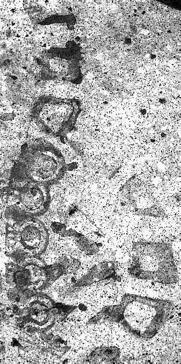
\includegraphics[width=\textwidth]{3/00009.jpg}
  \end{subfigure}
  \begin{subfigure}[b]{0.24\columnwidth}
    \centering
    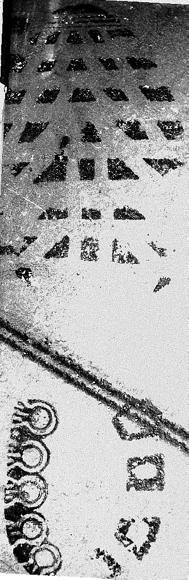
\includegraphics[width=\textwidth]{3/00020.jpg}
  \end{subfigure}
  \begin{subfigure}[b]{0.24\columnwidth}
    \centering
    \includegraphics[width=\textwidth]{3/00021.jpg}
  \end{subfigure}
  \begin{subfigure}[b]{0.24\columnwidth}
    \centering
    \includegraphics[width=\textwidth]{3/00066.jpg}
  \end{subfigure}
  \caption{Example impressions of the same shoe from the FID-300 \cite{kortylewski2014unsupervised} dataset}
  \label{fig:pe:database}
\end{figure}

\par
For that reason a discriminative feature learning algorithm is proposed based on the work of Guo et al. \cite{guo2012discriminative}.
In their work a three-layered Local Binary Pattern (LBP) feature learning algorithm is introduced for natural texture description, a schematic flow f the algorithm is shown on Figure \ref{fig:pe:workflow}
They utilize on feature selection where only the most discrimanitve descriptors are selected and propagated further.
In the first layer, where robustness is granted, the features which describe the majority of given texture are selected, by finding the frequently appearing features and ignoring the rare ones since they are more sensitive to noise.
For that a threshold is defined, all descriptors of the given texture are ordered by their frequency and selected in this order starting with the most frequent one.
If the already selected descriptors cover a bigger region of the original texture than the given threshold, the selection process stops and the chosen descriptors are proagated for the next level.
The selection of threshold is crucial in this process, if it is too high less robust descriptors with low frequency are also selected, when the threshold is too low, only the most frequent descriptors are considered and valuable details of the texture are ignored.

\begin{figure}[h]
  \centering
  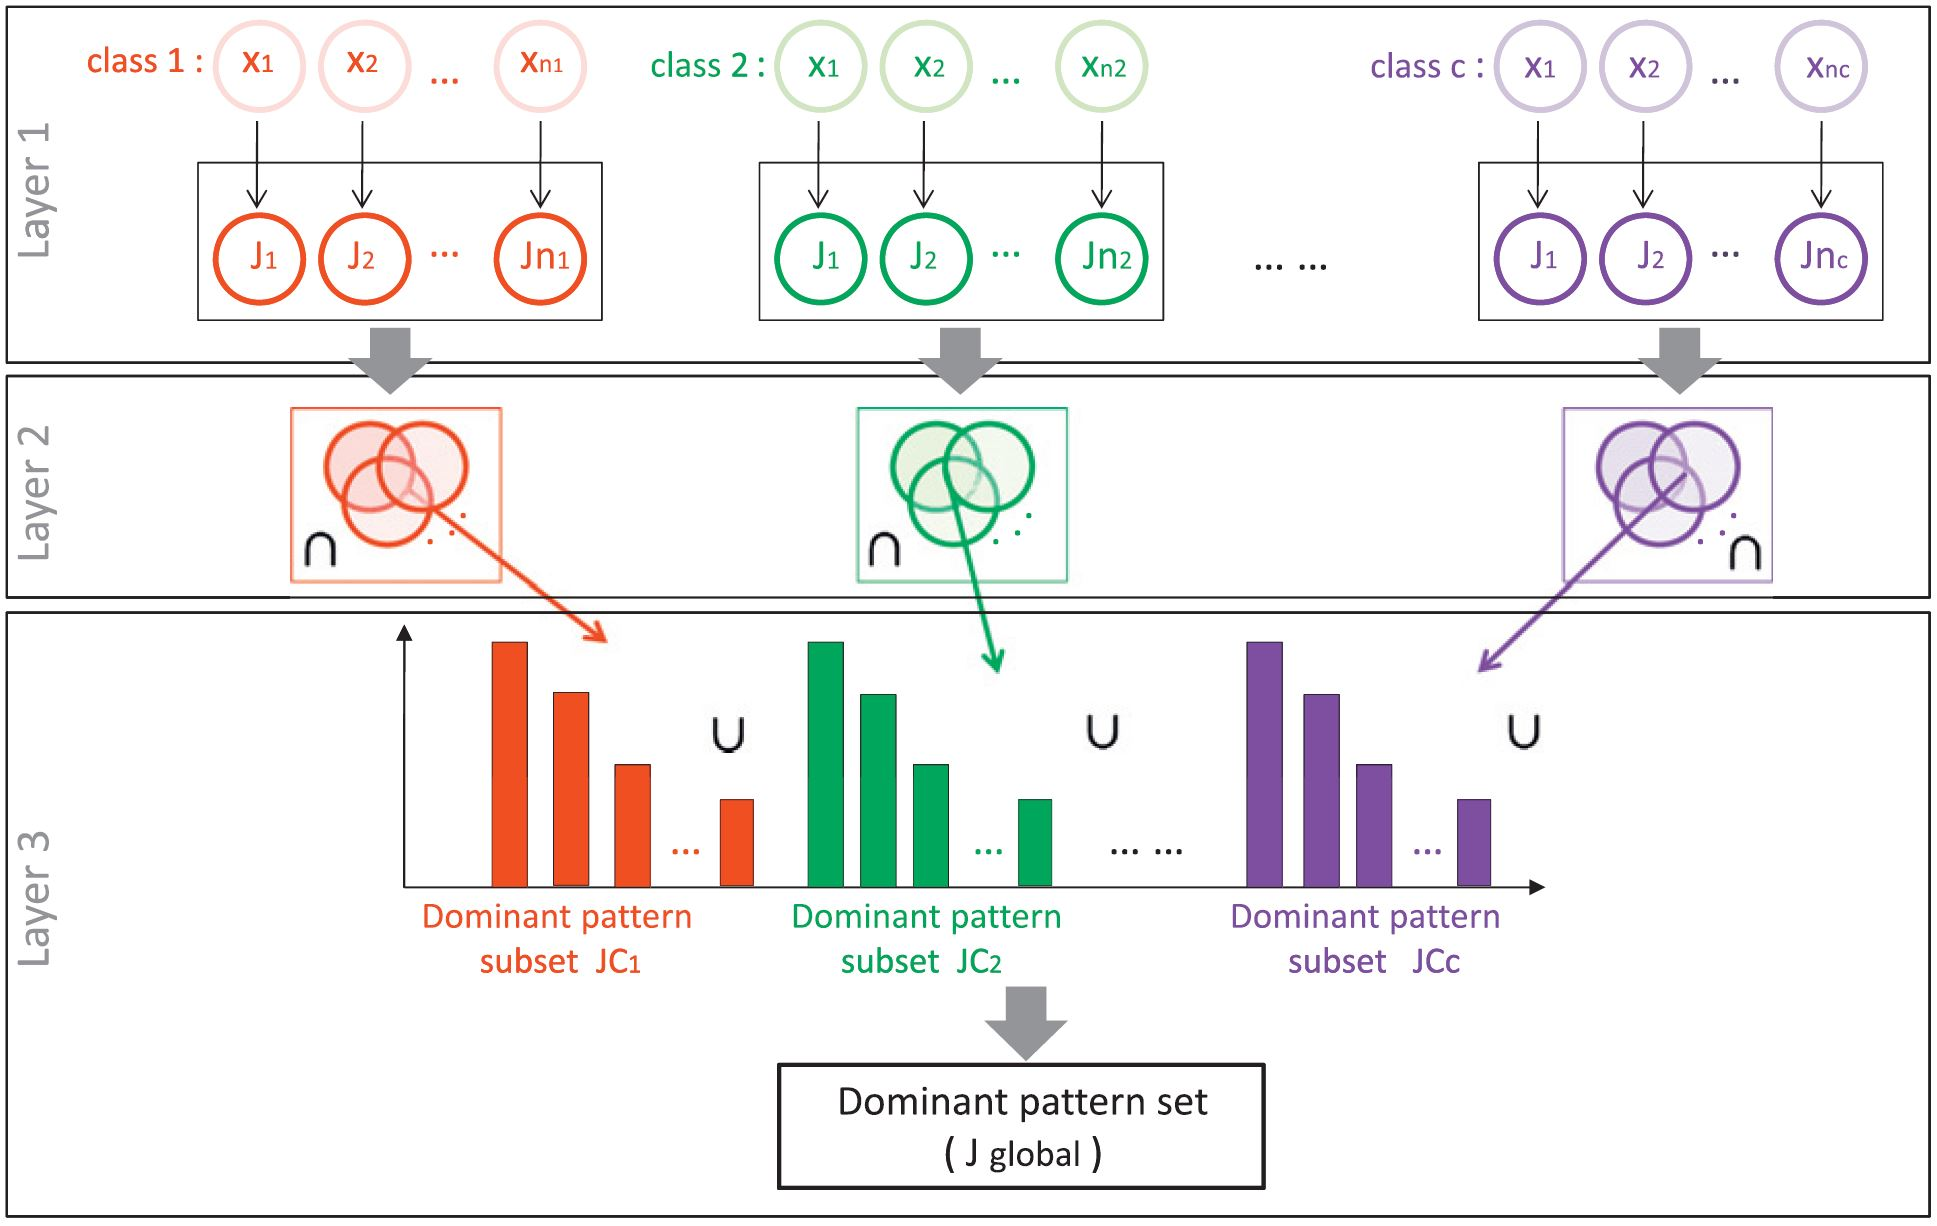
\includegraphics[width=\textwidth]{3/workflow.jpg}
  \caption{The workflow of the three-layered feature learning algorithm  \cite{guo2012discriminative}.}
  \label{fig:pe:workflow} % \label has to be placed AFTER \caption (or \subcaption) to produce correct cross-references.
\end{figure}

\par
The following two layers work according to Fisher\'s Separation Criteria, the second layer aims to minimize intra-class variance, whereas the third layer ensures maximum intra-class distance. 
The second layer provides discriminative power.
It gathers all selected descriptors from the previous layer of the same texture on different samples and intersects those sets.
The main assumption is that the same texture have similar properties under varying circumstances.
In this layer only the features are selected which occur in every sample of the given texture.
\par
In the last, third layer representation capability is ensured.
This layer merges all remaining features from the second layer into one set to create a dominant feature pool.
In the second layer a feature set for a given texture is created based on the extracted descriptors from all samples of the same texture, in the third layer those feature sets of every occuring textures are gathered and united.
\par
For the purpose of this prototypical implementation only the first two layer is used because the goal is to distinguish between noise and information.
The primary assumption is that there is a fundamental similarity between every shoeprint image, e.g. regualar line structures, reoccuring basic patterns, which can be detected and learned.
Guo et al. \cite{guo2012discriminative} proposed their algorithm for LBP features, and since it is popular descriptor for natural textures \cite{hong2014combining}, \cite{ahonen2009rotation} and fingerprints \cite{wang2013pixel}, \cite{rida2018palmprint}, LBP is chosen to be a candidate descriptor for shoeprint detection.
In the research of shoeprint identification both frequency based feture descriptors, such as Fourier-Mellin Transform \cite{wu2019crime}, \cite{gueham2008automatic}, and SIFT \cite{nibouche2009rotation}, \cite{richetelli2017classification} are commonly used descriptors, thus those are also selected for feature learning.
\par
The three-layered learning algorithm is implemented for three different feature descriptors, LBP, Fourier-Mellin and SIFT, but the learning process follows the same steps as proposed by Guo et al. \cite{guo2012discriminative}.
In the first layer Guo et al. \cite{guo2012discriminative} propose a threshold based on the area the selected features cover on the original image.
However this criteria is altered in the case of LBP and SIFT to adjust the learning algorithm to the needs of this research.
Three-layered learning was developed originally to find a discriminative feature set for several texture images from a wide database, from \cite{ojala2002outex}, \cite{dana1999reflectance}, \cite{boland2001neural}, \cite{jantzen2005pap} and \cite{brahnam2007introduction}, but in this project no such dataset is available.
Furthermore the goal is to distinguish between noise and soeprint and not to find discriminative features within multiple texture images.
For that reason features are firstly extracted from both fore- and background of the samples, where the foreground contains the exact shoeprint pattern and the background is the noisy ground where the shoeprint is lying.
Since there is no labelled data in the FID-300 \cite{kortylewski2014unsupervised} dataset available, the samples chosen for training were labelled manually.
Figure \ref{fig:pe:mask} shows two example images the black regions of the mask show the shoeprint information whereas the white pixels indicate the background.
After that, to achive high intra-class distnace despite the absence of the third layer, frequent descriptors of the noise are determined and all of them are eliminated from the pattern descriptors.
The remaining pattern descriptors are propagated to the next level. 
To have a reasonable learning time in case of Fourier-Mellin Transform no such modification is made.
After all descriptors are calculated those are selecte which occarancy exceed a given thresholds.

\begin{figure}[h]
  \centering
  \begin{subfigure}[b]{0.24\columnwidth}
    \centering
    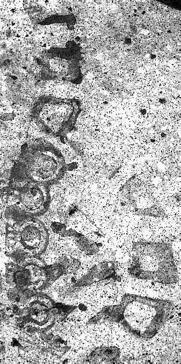
\includegraphics[width=\textwidth]{3/00009.jpg}
  \end{subfigure}
  \begin{subfigure}[b]{0.24\columnwidth}
    \centering
    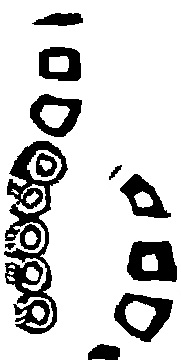
\includegraphics[width=\textwidth]{3/00009_mask.jpg}
  \end{subfigure}
  \begin{subfigure}[b]{0.24\columnwidth}
    \centering
    \includegraphics[width=\textwidth]{3/00025.jpg}
  \end{subfigure}
  \begin{subfigure}[b]{0.24\columnwidth}
    \centering
    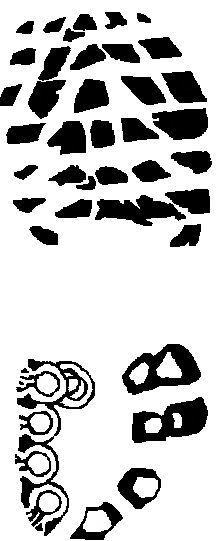
\includegraphics[width=\textwidth]{3/00025_mask.jpg}
  \end{subfigure}
  \caption{Examples from FID-300 \cite{kortylewski2014unsupervised} dataset chosen for three-layered learning and their corresponding manually labelled masks.}
  \label{fig:pe:mask}
\end{figure}

\par
The easiest way to determine the occurances of one descriptor is to calculate the complete matches within one sample.
This method however results in high amount of descriptors with little number of occurancies.
For that reason a similarity measure is used for all three candidate features, if the similarity value reaches a predefined threshold the two descriptors are considered as same, they are merged and the number for occurance is incremented.
For LBP histogram correlation is used for comparison, for SIFT Brute-Force matcher is applied and for the Fourier-Mellin Transform the similarity measure proposed in \cite{gueham2008automatic} used.
The correlation coefficient between two Fourier-Mellin descriptors is given by:
\[ corr(FM_{1},FM_{2}) = \frac{\sum\limits_{m}\sum\limits_{n}(FM_{1mn}-\overline{FM_{1}})(FM_{2mn}-\overline{FM_{2}})}{\sqrt{(\sum\limits_{m}\sum\limits_{n}(FM_{1mn}-\overline{FM_{1}})^2)(\sum\limits_{m}\sum\limits_{n}(FM_{2mn}-\overline{FM_{2}})^2)}}  \]
\label{FMcorr}
where $FM_{1}$ and $FM_{2}$ are two Fourier-Mellin Features to compare and $\overline{FM_{1}}$ and $\overline{FM_{2}}$ are the mean values of the corresponding features.
\par
At the end of the learning process a descriptor pool is created.
The shoeprint area of a new input is determined based on those learnt feature using the same similarity measures as in the learning phase.

\section{Implementation}
\par
In this section implementation details of the modified three-layered learning algorithms are revield and parameter settings are specified.
This and the following algorithms are written in Python 2.7 \cite{van1995python} using OpenCV 4.1.1 \cite{opencv_library}.
The values of the variables stated in this section are determined through experiments.
\par
When starting the application the training data is read.
It consists of the original shoeprint images and a mask image where the relevant regions of the corresponding shoeprint is marked.]
The two set of images are stored in a vector, it is assumed that the mask has the exact same size as the corresponding shoeprint image, that every image has a mask and that the images and masks are stored in the same order.
For training a limited amount of seven images were selected and labelled manually.
The FID-300 \cite{kortylewski2014unsupervised} dataset consists of 300 real-life forensic samples and 1175 synthetic samples, thus not every synthetic sample has a real pair, and the majority of synthetic images with corresponding real samples have only one or two matching pairs in the database.
The chosen seven images depict shoeprint images from the same shoe, one of them is a synthetic sample the rest of them is a real one.
\par
To speed up the shoeprint recognition, the learnt features are stored in a \texttt{.txt} file.
It is determined if a new learning process starts or the already determined descriptors are read from file.
When the learning starts the descriptors for all pixels are calculated.
For the Fourier-Mellin calculation the images are extended by mirroring the edges to have a uniform-sized (5x5) descriptor in all cases.
For LBP features two different settings are considered, one with radius of 3 and 12 sample points and one with radius of 5 and 24 sample points.
After that similar descriptors are merged and their frequency is calculated.
If the histogram correlation of two LBP features is higher than 90\%, if the distance between two SIFT features is lower than 300 and if the correlation between two Fourier-Mellin features is higher than 1.4 the two descriptors are combined.
After that the most frequent noise descriptors are determined, occuring at least 100 times among LBP and at least 10 times among SIFT features.
All LBP and SIFT descriptors are eliminated which have higher than 90\% correlation with and smaller than 250 distance to any dominant noise descriptor.
The remaining features are then propagated to the next layer.
In case of Fourier-Mellin Transform all descriptors are selected which occur at least 10 times on the given pattern.
\par
In the sceond layer the dominant descriptors of multiple samples are compared.
If there is a feature in every training images with a high enough similarity the feature is chosen and added to the final descriptor pool.
If the correlation between two LBP decsriptor is higher that 90\%, the distance between two SIFT features is smaller than 450 and the correlation between two Fourier-Mellin features is higher than 1.4, the feature is chosen and added to the final set of descriptor.
At the end of this process the whole set of descriptor is written into file.
\par
If the learned descriptors are available the input image is processed.
The descriptors of the input image are determined similarly as in the training phase.
For every pixel of the input is a descriptor calculated, in case of Fourier-Mellin transform the borders of the input are extended by mirroring.
The output image is calculated by comparing the descriptors of the input with the ones in the descriptor pool.
In case of LBP and Fourier-Mellin features the correlation value is simply written into the resulting image which is normalized in the end of calculation.
The result image of the SIFT feature comparison is binary, it is set to one if the descriptor of the corresponding pixel has a smaller distance than 200 to any descriptor from the learned set.
At the end of the application the resulting images are saved.

\section{Evaluation}
\par
In this section the results of the modified three-layered learning algorithm are presented and discussed.
Furthermore it is examined, if this approach can be used for real shoeprint identification algorithms.
\par
Two kind of experiments were conducted to test the performance of the learned descriptors.
First images from training data are evaluated to see how many descriptors from the original image were eliminated and to see the common featuers in the training dataset.
After that new images are set as input to examine if the features learned on one kind of data are able to describe other kind of shoeprint as well.
Figure \ref{fig:pe:25} and Figure \ref{fig:pe:66} are example images from the first scenario, since Figure \ref{fig:pe:25:orig} and Figure \ref{fig:pe:66:orig} are part of the training set.
The visible difference between Figure \ref{fig:pe:25:LBPs} and Figure \ref{fig:pe:25:LBPb} as well as between Figure \ref{fig:pe:66:LBPs} and Figure \ref{fig:pe:66:LBPb} shows that bigger radius is a better choice for shoeprint description.
Considering the middle region of Figure \ref{fig:pe:25}, the background on Figure \ref{fig:pe:25:LBPb} is less noisy than on Figure \ref{fig:pe:25:LBPs}.
This difference is more outstanding on  Figure \ref{fig:pe:66} where on Figure \ref{fig:pe:66:LBPs} no shoeprint can be recognized meanwhile on Figure \ref{fig:pe:66:LBPb} outlines of the pattern are visible.
Still focusing on the middle area of Figure \ref{fig:pe:25}, Figure \ref{fig:pe:25:SIFT} shows that the SIFT descriptor is similarly robust against noise as the LBP descriptor.
However, examining Figure  \ref{fig:pe:25:FM} the Fourier-Mellin descriptor has more difficulties with the same area, where the background is less homogen than on  Figure \ref{fig:pe:25:LBPb} and on Figure \ref{fig:pe:25:SIFT}.
On the other hand, inspecting the bottom left side of the shoeprint, it can be seen that the Fourier-Mellin features menaged to find the whole area of pattern, whereas only a few outlines are recognizable on Figure \ref{fig:pe:25:LBPb} and on Figure \ref{fig:pe:25:SIFT}.
Intrestingly that said region is more recognozable on  \ref{fig:pe:66:LBPs} than on  \ref{fig:pe:66:LBPb}.
Based on these observations it can be stated that the features less robust against noise are able to find a higher portion of pattern area than those with higher robustness.
In exchange the background area stays still noisy and further image processing is needed.
Comparing all results of the two images, Figure \ref{fig:pe:25} and Figure \ref{fig:pe:66}, the performance strongly depends on the input quality.
On Figure \ref{fig:pe:66} and Figure \ref{fig:pe:66:SIFT} the pattern is less recognizable than on the previous example and a higher amout of background pixels are labeled as pattern.
On cluttered images Fourier-Mellin features seem to outperform both SIFT and LBP descriptors.
Overall this testing scenario shows ambivalent results.
On the one hand on clear samples LBP and SIFT fis able to distinguish between fore- and background correctly, on the other hand, if the input data is cluttered those two descriptors are barely able to recognize the pattern and the Fourier-Mellin descriptor provides the clearest resulst. 

\begin{figure}[h]
  \centering
  \begin{subfigure}[b]{0.19\columnwidth}
    \centering
    \includegraphics[width=\textwidth]{3/00025.jpg}
    \subcaption{Example image from the training set}
    \label{fig:pe:25:orig}
  \end{subfigure}
  \begin{subfigure}[b]{0.19\columnwidth}
    \centering
    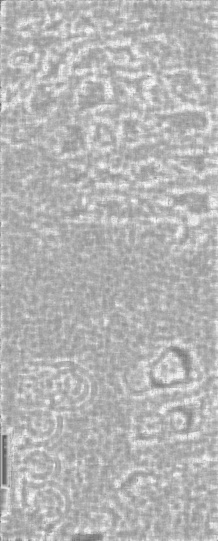
\includegraphics[width=\textwidth]{3/LBP/output_00025.jpg}
    \subcaption{Output using LBP descriptors with radius 3 and 12 sample points}
    \label{fig:pe:25:LBPs}
  \end{subfigure}
  \begin{subfigure}[b]{0.19\columnwidth}
    \centering
    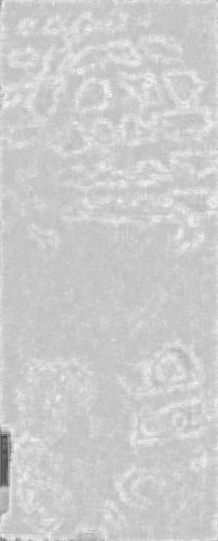
\includegraphics[width=\textwidth]{3/LBP/output_00025_6_24_5.jpg}
    \subcaption{Output using LBP descriptors with radius 5 and 24 sample points}
    \label{fig:pe:25:LBPb}
  \end{subfigure}
  \begin{subfigure}[b]{0.19\columnwidth}
    \centering
    \includegraphics[width=\textwidth]{3/FM/00025.jpg}
    \subcaption{Output using Fourier-Mellin Descriptor}
    \label{fig:pe:25:FM}
  \end{subfigure}
  \begin{subfigure}[b]{0.19\columnwidth}
    \centering
    \includegraphics[width=\textwidth]{3/SIFT/00025.jpg}
    \subcaption{Output using SIFT Descriptor}
    \label{fig:pe:25:SIFT}
  \end{subfigure}
  \caption{Output of the modified three-layered learning algorithm on an image from training set}
  \label{fig:pe:25}
\end{figure}

\begin{figure}[h]
  \centering
  \begin{subfigure}[b]{0.19\columnwidth}
    \centering
    \includegraphics[width=\textwidth]{3/00066.jpg}
    \subcaption{Example image from the training set}
    \label{fig:pe:66:orig}
  \end{subfigure}
  \begin{subfigure}[b]{0.19\columnwidth}
    \centering
    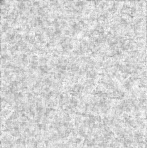
\includegraphics[width=\textwidth]{3/LBP/output_00066_4_12_3.jpg}
    \subcaption{Output using LBP descriptors with radius 3 and 12 sample points}
    \label{fig:pe:66:LBPs}
  \end{subfigure}
  \begin{subfigure}[b]{0.19\columnwidth}
    \centering
    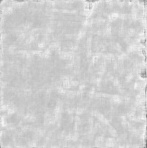
\includegraphics[width=\textwidth]{3/LBP/output_00066_6_24_5.jpg}
    \subcaption{Output using LBP descriptors with radius 5 and 24 sample points}
    \label{fig:pe:66:LBPb}
  \end{subfigure}
  \begin{subfigure}[b]{0.19\columnwidth}
    \centering
    \includegraphics[width=\textwidth]{3/FM/00066.jpg}
    \subcaption{Output using Fourier-Mellin Descriptor}
    \label{fig:pe:66:FM}
  \end{subfigure}
  \begin{subfigure}[b]{0.19\columnwidth}
    \centering
    \includegraphics[width=\textwidth]{3/SIFT/00066.jpg}
    \subcaption{Output using SIFT Descriptor}
    \label{fig:pe:66:SIFT}
  \end{subfigure}
  \caption{Output of the modified three-layered learning algorithm on an image from training set}
  \label{fig:pe:66}
\end{figure}

\par
On Figure \ref{fig:pe:182} the results of the modiefied three-layered learning algorithm on a non-training sample are shown.
The results displayed on Figure \ref{fig:pe:182:LBPs} and on Figure \ref{fig:pe:182:LBPb} strenghtens the observation, that bigger neighborhood LBP outperforms the smaller radius descriptor.
Furthermore examining the middle, noisy, part of the images in all three cases a homogenous background can be seen containing some falsely labelled pixels.
Observing the bottom part of the shoe a weakness of LBP and SIFT already discussed is noticable.
On the original image there are small structures which are part of the shoeprint.
Similarly as on the bottom left part of Figure \ref{fig:pe:25} the fine structures are only partially recognized, comparing Figure \ref{fig:pe:182:FM} to Figure \ref{fig:pe:182:LBPb} and to Figure \ref{fig:pe:182:SIFT} Fourier-Mellin outperfoms LBP and SIFT again labelling the whole area correctly.

\begin{figure}[h]
  \centering
  \begin{subfigure}[b]{0.19\columnwidth}
    \centering
    \includegraphics[width=\textwidth]{3/00182.jpg}
    \subcaption{Input image}
    \label{fig:pe:182:orig}
  \end{subfigure}
  \begin{subfigure}[b]{0.19\columnwidth}
    \centering
    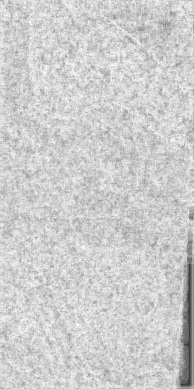
\includegraphics[width=\textwidth]{3/LBP/output_00182_4_12_3.jpg}
    \subcaption{Output using LBP descriptors with radius 3 and 12 sample points}
    \label{fig:pe:182:LBPs}
  \end{subfigure}
  \begin{subfigure}[b]{0.19\columnwidth}
    \centering
    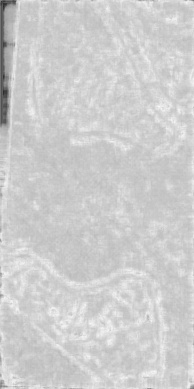
\includegraphics[width=\textwidth]{3/LBP/output_00182_6_24_5.jpg}
    \subcaption{Output using LBP descriptors with radius 5 and 24 sample points}
    \label{fig:pe:182:LBPb}
  \end{subfigure}
  \begin{subfigure}[b]{0.19\columnwidth}
    \centering
    \includegraphics[width=\textwidth]{3/FM/00182.jpg}
    \subcaption{Output using Fourier-Mellin Descriptor}
    \label{fig:pe:182:FM}
  \end{subfigure}
  \begin{subfigure}[b]{0.19\columnwidth}
    \centering
    \includegraphics[width=\textwidth]{3/SIFT/00182.jpg}
    \subcaption{Output using SIFT Descriptor}
    \label{fig:pe:182:SIFT}
  \end{subfigure}
  \caption{Output of the modified three-layered learning algorithm}
  \label{fig:pe:182}
\end{figure}

\par
To summarize LBP and SIFT features seem to be less responsive in the noisy area and have difficulties to find fine patterns while the Fourier-Mellin transform labels bigger parts of the actual shoeprint correctly whereas it more often mistakes the noise as foreground.
Based on the testing images Fourier-Mellin recognize the shoeprint pixels in nosiy images better than LBP and SIFT.
A possible solution is to combine all three feature descriptors and propose a weighting score across them, assuming that all three feature sets were able to provied usable results for further processing.
In ow quality images that is however not necessarily the case.
Even though Figure \ref{fig:pe:66} was part of the testing dataset, LBP and SIFT was not able to label the pattern correctly.
That problem can originate from the learning process, where all dominant descriptors of the noise part are eliminated from the pattern descriptors.
On the other hand on Figure \ref{fig:pe:66:SIFT} significant amount of background is labelled as pattern, which indicates that too many noise descriptors were selected into the descriptors pool.
Furthermore there are several lower quality samples in the whole dataset available then the one presented on Figure  \ref{fig:pe:66}.
It has to be emphasized that the descriptors were learned on a small dataset.
Incorporating more samples and altering the learning criteria, e.g. the given feature has to be found in a given ratio of training images and not on every one of them, can lead to a broader texture pool.
However, this can also result higher ratio of noise descriptors in the final feature set.
High noise ratio seems to be a limitation of this algorithm in its current form.
For that reason noise supression techniques are examined in the following two chapters.
In the future the three-layered learning algorithm can be further developed and used jointly with noise supression techniques to solve its weakness and to take advante on its possible performance.

\chapter{Fully Automated Noise Supression}

Since the algorithm introduced in the previous chapter had difficoulties when processing noisy or cluttered data two noise supression techniques are introduced now.
In this chapter a fully-automated in the following one a semi-automated approach is proposed.
Similar to the previous method the main goal is to distinguish between noise and pattern, but this time instead of finding pattern regardless the noise, the noise is suppressed first and the information is enhanched afterwards.
\par
To be able to compare the the proposed methods more easily, the structure of this chapter is the same as the previous one.
The methodology is discussed first, afterwards implementation details are given, finally the results are examined and evaluation of the method is discussed.

\section{Methodology}
\par
The method proposed in this chapter has three main steps, first the noise is supressed, after that the shoeprint pattern is enhanced and the result image is generated lastly by thresholding.
The flowchart of the entire algorithm is shown on Figure \ref{fig:fans:workflow}.

\begin{figure}[h]
  \centering
  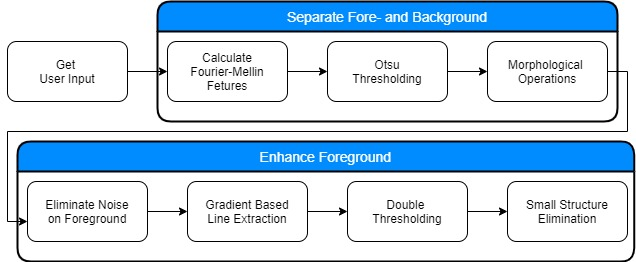
\includegraphics[width=\textwidth]{4/flow.jpg}
  \caption{The workflow of the fully automated noise suppression algorithm.}
  \label{fig:fans:workflow} % \label has to be placed AFTER \caption (or \subcaption) to produce correct cross-references.
\end{figure}

\par
The first part of the algorithm is responsible for noise suppression.
Since there is little research done on enhancement of real-life forensic images two filters proven to be effective in noise elimination are combined.
As Li et al. \cite{li2014rapid} state, Wiener filter is among the most popular techniques in the topic of noise reduction, the filter is however not able to reconstruct the signal data it only supresses the noise component.
Wiener filter works in the signal domain, where it estimates the original image based on the cluttered input. 
The filter is given by following Equation \cite{Win}:
\[ G(u, v) = \frac{H^*(u,v) P_s(u, v)}{\mid H(u,v)\mid ^2 P_s (u, v) + P_n (u, v)}  \]
where $H(u,v)$ stands for the Fourier transform of the point-spread function, $P_s (u,v)$ denotes the power transform of the signal, which is the Fourier Transform of the signal autocorrelation and $P_n(u,v)$ expresses the power spectrum of noise, which is the the Fourier Transform of the noise autocorrelation.
The performance of the filtering strongly depends on the quality of $P_s$, on the estimated appearance of the original image.
In this method it is estimated based on the input image.
The other method used for noise suppression is Bilateral Filtering as proposed in \cite{huang2013self} and in \cite{zhang2016simultaneous}.
Similar to the Wiener Filter Bilateral Filter is also used for smoothing the image, but since it considers the weighted average of neighboring pixels it preserves the edge information which is crucial to prevent blurring on the shoeprint pattern as well. 
When both images are calculated the difference of those two images is propagated.
In this way the blurring effect is strengthened in the background while the outlines of the shoeprint patterns are preserved.
\par
For enhanchement Successive Mean Quantization Transform (SMQT) \cite{nilsson2013smqt} is used as proposed by Katireddy et al. \cite{katireddy2017novel}.
SMQT is recursive algorithm which splits the data into two parts in every level depending on the current data value beeing smaller or bigger than the mean of the given data part.
In this way the structure of the data is exposed.
Everytime the image is separated into two parts, it is noted first which pixel is under (0) and which one is above (1) the current mean.
The algorithm then recurseviely continues on both subgroups of the images, splitting and noting the relative pixel value again.
Note that the pixels in the same subgroup does not have to be neighboring, the lustering is solely based on the illumination value.
The recursion stops if the predefined depth is achived.
To finish the transformation the noted cluster position values of the pixels are examined.
Along the levels of the recursion a sequence of ones and zeros are registered for every pixels.
As a last step this sequence is considered as a binary number and after converting into decimal value it is updated as the intensity of the corresponding pixel.
\par
The last part of the application is the postprocessing step where the input is converted into a binary image and small inconsistencies and remaining noise are eliminated.
When binarizing footprint images Otsu's technique \cite{algarni2008novel}, \cite{alizadeh2017automatic}, \cite{wu2019crime} or adaptive thresholding \cite{wang2014automatic} is used most frequently.
However in the proposed enhancement approach Niblack Binarization Method (NBM) \cite{niblack1985introduction} is preferred.
NBM is a local thresholding method and it can be calculated as follows \cite{saxena2019niblack}:
\[T_d = m(x,y) + k * s(k, y)\]
where $m$ and $s$ stands for mean and dtandard deviation in the given area respectively and $k$ is a configuration variable which is given manually. 
There are several publications available \cite{som2011application}, \cite{athimethphat2011review}, which prove that global methods, such as Otsu Thresholding \cite{otsu1979threshold}, is less fasible as their local counterparts.
Although the studies mentioned were carried out on text documents with varying image quality, the two domains can be considered as familiar since they both aim to find fine line structures on a cluttered background.
Furthermore, Saxena et al. \cite{saxena2019niblack} also state that NBM is one of the most powerful thresholding method, outperforming the global and some local tecniques as well. 
There is however one disadvatage of local binarization and that is local window size.
Since for every subwindow a new threshold is calculated NBM tends to generate salt and pepper noise on more homgenous, e.g. background, area.
For that reason two other postprocessing methods are also implemented.
The first one eliminates short lines on the image, based on the assumption that the actual shoepattern outlines are recognized and they build bigger, coherent edges.
The second algorithm is also stand on the same principle, from the remaining lines are all open structures eliminated unless the length is higher than a given threshold bigger than in the previous step.
It is based on the observation, that if the complete structure of a pattern element is found, since NBM concentrates on the contours, a closed line structure is extracted.
When there is no pattern element in a NBM subwindow only the edges of remaining clutter and binarization artifacts are generated.
Since those lines are most likely not closed, they are deleted.
It is however still possible, that an open line structure is generated if only parts of the shoeprint are classified correctly.
For that reason not every open edge, only a subgroup of them, which are shorter than a threshold, is eliminated.

\section{Implementation}
\par
Implementation details and parameter settings are discussed  in the followings.
The programming tools are similar to the ones in the previous chapter Python 2.7 \cite{van1995python} with OpenCV 4.1.1 \cite{opencv_library} were used for development.
Since all methods presented in this thesis all prototypical applications, the parameter settings were determined experimentally.
\par
At the start of the application the input image is read and frowarded to the denoising stage.
The original image is processed separatly with Wiener and Bilateral Filter.
To apply the Wiener Filter correctly the input image is normalized first for the range of 0 to 1.
For the Point Spread Function an image of size 5x5 is set.
The balance parameter is 1100 which sets the ratio between information adequcy and prior adequcy, those parameters control frequency increment and decrement respectively.
The kernel size onf the Bilateral Filter is 9x9.
When both filtered images are calculated their difference is determined and propagated to the enhancement step of the algorithm.
\par
For SMQT calculation, for save time, a speeded up version is implemented.
In the first step a table of occuring values on the image is created where the zeroth column corresponds the pixel value of 0, the first column stands for pixel value of 1 and so on.
In the first row of the table the frequency of the given value is noted, that is the number of pixels having the value which the column corresponds with.
In the second row the sum of frequencies up to the current column is stored.
The third row represents the sum of all elements until the given column.
This table eases the calculation of mean value for every level of the SMQT algorithm.
Additionally, since the enties are ordered, if the subgrouping starts, the values belonging to the same cluster will be neighboring columns.
Figure \ref{fig:fans:table} shows the frist 14 colums of the occurancy map of an example image.
When the occaurancy map is ready the recursion starts, the mean of the given subgroup is determined and splitted into two parts according to the pixel value of the given column beeing bigger or smaller than the mean value. 
Every column of the table have a binary code which is created during the recursion.
In the first level the first digit of the code is written, in the second level the second digit etc. the length of this code is the same as the predefined depth of the recursion.
If a pixel value is smaller or equal to the calculated mean of the given cluster a zero is written in the belonging binary code, and a 1 is recorded if it is bigger.
The manually set depth of the recursion is 8, in this way when the final binary codes are converted to a decimal number a range of 0 to 255 is covered.
\begin{figure}[h]
  \centering
  \begin{subfigure}[b]{0.09\columnwidth}
    \centering
    \includegraphics[width=\textwidth]{4/21/00021.jpg}
  \end{subfigure}
  \begin{subfigure}[b]{0.9\columnwidth}
    \centering
    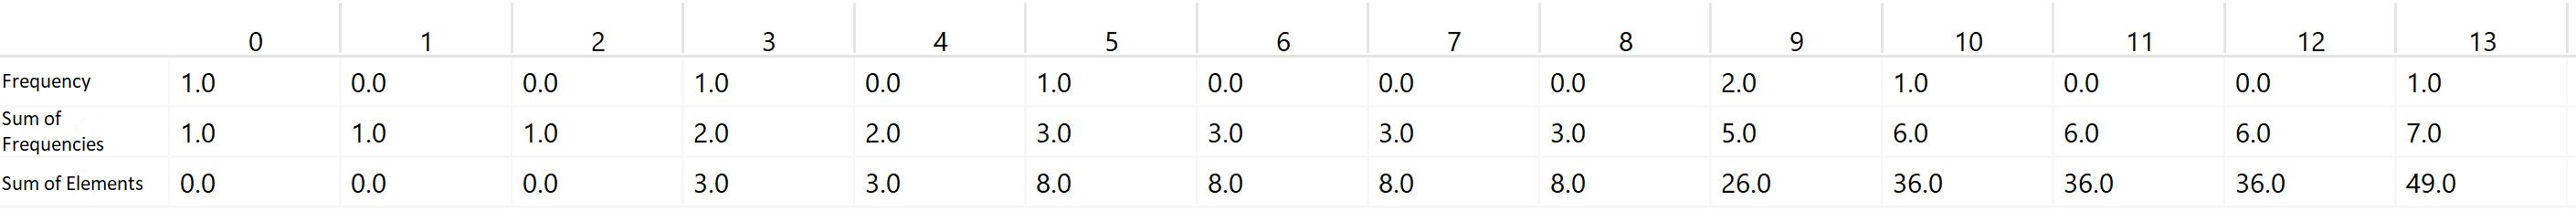
\includegraphics[width=\textwidth]{4/table.jpg}
  \end{subfigure}
  \caption{The first 14 columns of the occurancy map. The header of the table represents the possible pixel values. }
  \label{fig:fans:table} % \label has to be placed AFTER \caption (or \subcaption) to produce correct cross-references.
\end{figure}
\par
In the last step the image is thresholded according to NBM.
The window size is the same as the size of the Winwe Filter, 5x5.
Furthermore the regularization parameter $k$ of NBM is set to 0.5.
After that short and non-long edges are eliminated.
The connected components of the image are extrcted first considering 8-neighborhood.
After that every component is examined on their size and if they are smaller than a given threshold they are deleted.
It is possible to set the threshold to the average size of every regions, however experimental results show that a such high criterion eliminate shoepattern lines as well.
For that reason a manually set threshold is used, which is set to 50 for every test images.
The short line elimination algorithm is applied on both the fore- and on the background on the image.
Lastly the remaining components are examined on ther openness.
If an open line structure is found which overall lengths is smaller than a manually set threshold it is deleted.
This threshold is set to be 60 during the whole experiment.

\section{Evaluation}
\par
In the following section the experimental results are presented.
Furthermore the performance and the usability of the proposed algoritm is also discussed.
Figures \ref{fig:fans:denoise} and \ref{fig:fans:enhance} the output of the proposed algorithm on every stages and presents the final results as well.
\par
Figure \ref{fig:fans:denoise} shows the output of the denoising pipeline on three example images from the FID-300 database.
In the second column the Wiener filtered images are shown, in the third one the Bilateral filtered images whereas the differene etween those two images is in the las row.
Considering the background of the algorithms and the amount of noise on the images only a light smoothing is done in the denoising phase.
This decision was made to protect the valuable pattern information.
Since no previous knowledge is available abot the properties of shoeprint, no agressive filter kernel is used to make sure that the relevant information is preserved correctly.
On the combined image a bright silhoutte around the shoeprint image is visible, which was created by the Wiener filter.
This feature is exploited in a later stage of the algorithm, where an edge sensitive binarization method is used.

\begin{figure}[h]

\subfloat{
  \centering
  \begin{subfigure}[b]{0.24\columnwidth}
    \centering
    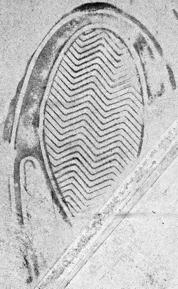
\includegraphics[width=\textwidth]{4/241/00241.jpg}
    \subcaption{Example image}
    \label{fig:fans:241:orig}
  \end{subfigure}
  \begin{subfigure}[b]{0.24\columnwidth}
    \centering
    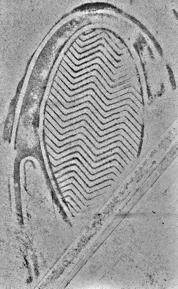
\includegraphics[width=\textwidth]{4/241/00241_wiener.jpg}
    \subcaption{Wiener filtered image}
    \label{fig:fans:241:wiener}
  \end{subfigure}
  \begin{subfigure}[b]{0.24\columnwidth}
    \centering
    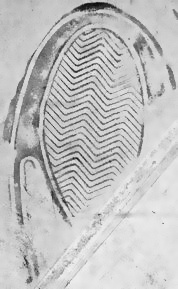
\includegraphics[width=\textwidth]{4/241/00241_bi5.jpg}
    \subcaption{Bilateral filtered image}
    \label{fig:fans:241:bi}
  \end{subfigure}
  \begin{subfigure}[b]{0.24\columnwidth}
    \centering
    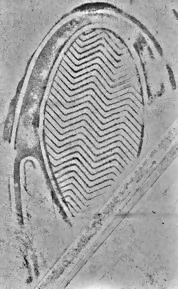
\includegraphics[width=\textwidth]{4/241/00241_denoise.jpg}
    \subcaption{Denoised image}
    \label{fig:fans:241:denoise}
  \end{subfigure}
  \label{}
}

\subfloat{
    \centering
  \begin{subfigure}[b]{0.24\columnwidth}
    \centering
    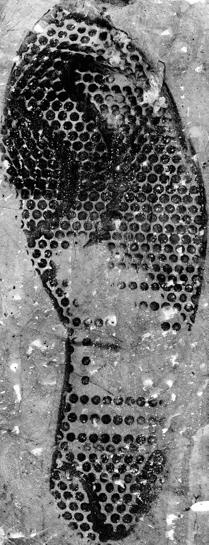
\includegraphics[width=\textwidth]{4/235/00235.jpg}
    \subcaption{Example image}
    \label{fig:fans:235:orig}
  \end{subfigure}
  \begin{subfigure}[b]{0.24\columnwidth}
    \centering
    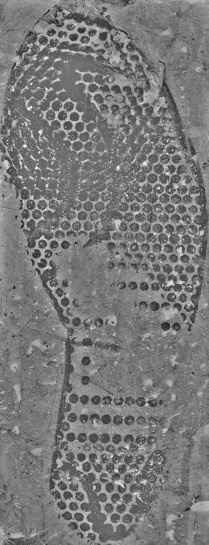
\includegraphics[width=\textwidth]{4/235/00235_wiener.jpg}
    \subcaption{Wiener filtered image}
    \label{fig:fans:235:wiener}
  \end{subfigure}
  \begin{subfigure}[b]{0.24\columnwidth}
    \centering
    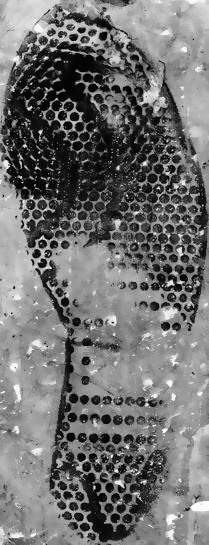
\includegraphics[width=\textwidth]{4/235/00235_bi5.jpg}
    \subcaption{Bilateral filtered image}
    \label{fig:fans:235:bi}
  \end{subfigure}
  \begin{subfigure}[b]{0.24\columnwidth}
    \centering
    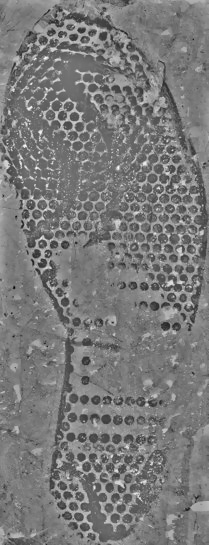
\includegraphics[width=\textwidth]{4/235/00235_denoise.jpg}
    \subcaption{Denoised image}
    \label{fig:fans:235:denoise}
  \end{subfigure}
}

\subfloat{
  \centering
  \begin{subfigure}[b]{0.24\columnwidth}
    \centering
    \includegraphics[width=\textwidth]{4/21/00021.jpg}
    \subcaption{Example image}
    \label{fig:fans:21:orig}
  \end{subfigure}
  \begin{subfigure}[b]{0.24\columnwidth}
    \centering
    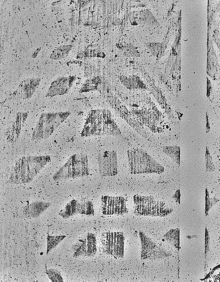
\includegraphics[width=\textwidth]{4/21/00021_wiener.jpg}
    \subcaption{Wiener filtered image}
    \label{fig:fans:21:wiener}
  \end{subfigure}
  \begin{subfigure}[b]{0.24\columnwidth}
    \centering
    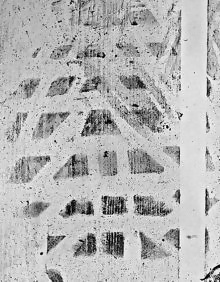
\includegraphics[width=\textwidth]{4/21/00021_bi5.jpg}
    \subcaption{Bilateral filtered image}
    \label{fig:fans:21:bi}
  \end{subfigure}
  \begin{subfigure}[b]{0.24\columnwidth}
    \centering
    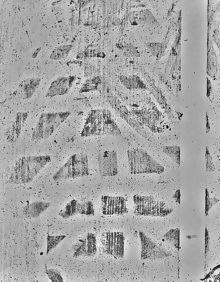
\includegraphics[width=\textwidth]{4/21/00021_denoise.jpg}
    \subcaption{Denoised image}
    \label{fig:fans:21:denoise}
  \end{subfigure}
}

\caption{Example for the results of the denoising stage}
\label{fig:fans:denoise}

\end{figure}

\par
The second step of the algorithm is enhancement where SMQT is applied, and the results are shown on Figures \ref{fig:fans:241:enhance}, \ref{fig:fans:235:enhance} and \ref{fig:fans:21:enhance}.
The benefit is the SMQT algorithm is ambiguous.
On the one hand focusing on the middle area of Figures  \ref{fig:fans:241:enhance} and \ref{fig:fans:235:enhance} the difference between fore- and background is bigger than on the original image.
The contours of the shoeprint are more outstanding than on the original image.
Furthermore the halo effect is also more visible than on the output of the previous sage of the algorithm.
Comparing Figure \ref{fig:fans:235:enhance} to Figure \ref{fig:fans:21:denoise}, the shoepattern structures got darker and there is a brighter area around the contours than on Figure \ref{fig:fans:21:denoise}.
On the other hand not only the information but also the remaining noise elements got enhanced by SMQT.
Even thoug the denoising stage is finished, since only moderate smoothing was applied, there is a considerable noise on the input images for SMQT.
The soft filtering is able to cope with Gaussian noise like on Figure \ref{fig:fans:241:denoise} but it does not eliminate bigger clutter particles like on the left side of Figure \ref{fig:fans:235:denoise} or on the upper region of Figue \ref{fig:fans:21:denoise}.
The SMQT enhancement makes those clutter more obvious by increasing the color difference between the noise and the homogenous background, for example the already mentioned patches on the left side of Figure \ref{fig:fans:235:denoise} are now more visible than on the original image \ref{fig:fans:235:orig}.
Additionally SMQT has similar effect like Histogram Equalization, the background on Figure \ref{fig:fans:241:denoise} is near homogenous, but after applying SMQT its color changes are more obvious since the original pixel values are mapped now to a wider color range.

\begin{figure}[h]

\subfloat{
  \centering
  \begin{subfigure}[b]{0.24\columnwidth}
    \centering
    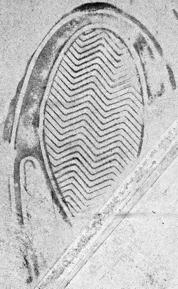
\includegraphics[width=\textwidth]{4/241/00241.jpg}
    \subcaption{Example image}
  \end{subfigure}
  \begin{subfigure}[b]{0.24\columnwidth}
    \centering
    \includegraphics[width=\textwidth]{4/241/00241_enhnace.jpg}
    \subcaption{Enhanced image}
    \label{fig:fans:241:enhance}
  \end{subfigure}
 \begin{subfigure}[b]{0.24\columnwidth}
    \centering
    \includegraphics[width=\textwidth]{4/241/00241_threshold.jpg}
    \subcaption{Binarized image}
    \label{fig:fans:241:bin}
  \end{subfigure}
  \begin{subfigure}[b]{0.24\columnwidth}
    \centering
    \includegraphics[width=\textwidth]{4/241/00241_result.jpg}
    \subcaption{Output image}
    \label{fig:fans:241:out}
  \end{subfigure}
}

\subfloat{
    \centering
  \begin{subfigure}[b]{0.24\columnwidth}
    \centering
    \includegraphics[width=\textwidth]{4/235/00235.jpg}
    \subcaption{Example image}
  \end{subfigure}
  \begin{subfigure}[b]{0.24\columnwidth}
    \centering
    \includegraphics[width=\textwidth]{4/235/00235_enhnace.jpg}
    \subcaption{Enhanced image}
    \label{fig:fans:235:enhance}
  \end{subfigure}
 \begin{subfigure}[b]{0.24\columnwidth}
    \centering
    \includegraphics[width=\textwidth]{4/235/00235_threshold.jpg}
    \subcaption{Binarized image}
    \label{fig:fans:235:bin}
  \end{subfigure}
  \begin{subfigure}[b]{0.24\columnwidth}
    \centering
    \includegraphics[width=\textwidth]{4/235/00235_result.jpg}
    \subcaption{Output image}
    \label{fig:fans:235:out}
  \end{subfigure}
}

\subfloat{
  \centering
  \begin{subfigure}[b]{0.24\columnwidth}
    \centering
    \includegraphics[width=\textwidth]{4/21/00021.jpg}
    \subcaption{Example image}
  \end{subfigure}
  \begin{subfigure}[b]{0.24\columnwidth}
    \centering
    \includegraphics[width=\textwidth]{4/21/00021_enhnace.jpg}
    \subcaption{Enhanced image}
    \label{fig:fans:21:enhance}
  \end{subfigure}
 \begin{subfigure}[b]{0.24\columnwidth}
    \centering
    \includegraphics[width=\textwidth]{4/21/00021_threshold.jpg}
    \subcaption{Binarized image}
    \label{fig:fans:21:bin}
  \end{subfigure}
  \begin{subfigure}[b]{0.24\columnwidth}
    \centering
    \includegraphics[width=\textwidth]{4/21/00021_result.jpg}
    \subcaption{Output image}
    \label{fig:fans:21:out}
  \end{subfigure}
}

\caption{Example for the results of the enhancement and postprocessing stage}
\label{fig:fans:enhance}

\end{figure}

\par
The closing step of the algorithm is postprocessing, consisting of binarization (the thrid column of Figure \ref{fig:fans:enhance}) and line-clutter elimination (in the fourth column of Figure \ref{fig:fans:enhance}).
As expected NBM is able to take advantage on the halo effect and finds the shoepattern correctly. 
On all three images, Figure \ref{fig:fans:241:bin}, Figure \ref{fig:fans:235:bin} and Figure \ref{fig:fans:21:out}, the contours of the patterns are clearly visible.
However, the drawbacks of NBM and the enhanced noise by SMQT are evident, since among the correct outline edges a high amount of noise is generated.
For that reason the closing step of short line and open line structure elimination is executed.
On Figures \ref{fig:fans:241:out} and \ref{fig:fans:235:out} the majority of background is cleared up and the shoeprint pattern is showed correctly.
On the other hand on Figure \ref{fig:fans:21:out} the original pattern is not recognizable anymore, along with the background noise relevant contour edges were also eliminated, and noise lines attached to the shoeprint pattern were kept.
\par
This presented results of the fully-automated noise suppression algorithm indicate two things.
First NBM with the current postprocessing tecnique works better on samples with fine lines, Figure \ref{fig:fans:241:orig}, and with detailed small structures, Figure \ref{fig:fans:235:orig}.
As already discussed and shown NBM tends to generate line noise on homogenous areas, if the shoeprint consist of dense pattern, there is no big, homogenous background between the different structure elements thus no noise is generated.
Additionally the heuristics which the two postprocessing steps are based on do not apply on every samples on the database.
On Figure  \ref{fig:fans:21:bin} even though there is a high amount of noise the pattern is clearly recognizable whereas on Figure \ref{fig:fans:21:out} no shoeprint can be seen anymore.
This implies that the settings of the line elimination algorithms are not correct and that further postprocessing is needed
Several pattern edges were eliminated because they were too short.
The threshold for line length were not changed during testing, thus a possible solution for the problem is to always adjust the parameter according to the current image.
This adjustment is however difficult since there is no a-priori knowledge about the sample available.
Alternatively looking to Figure  \ref{fig:fans:21:out} the outlines of the pattern were found originally, but becuase of noise they were not connected.
In the application 8-neighborhood is considered, but the connectivity-criteria can be extended.
But this causes more connectivity among noise as well.
Furthermore it also magnifies the second problem occuring on Figure \ref{fig:fans:21:out}, that noise lines are connected to the contours, thus are not eliminated.
An additional postprocessing step is needed to examine the remaining edges and determine which connection was made unintenionally.
\par
Second, Figures \ref{fig:fans:235:out} and \ref{fig:fans:21:out} show that the performance of fully-automated noise suppression algorithm strongly depends on the quality of the input image.
This algorithm has a similar limitation like the modified three-layered learning approach proposed in the previous chapter.
Initially the filter settings of the denoising step are not able to handle cluttered noise seen on Figures \ref{fig:fans:235:orig} and \ref{fig:fans:21:orig}.
Chatterjee et al. \cite{chatterjee2011patch} proposed a method which represents the estimated image for Wiener filter based on geometrically and photometrically similar regions.
Even though their approach had promising results, it was tested on data with Gaussian noise and not with irregular cluttered noise seen on the majority if FID-300 images.
Later, in the enhancement step not only the information but the remaining noise elements are also enhanced.
Lastly, during binarization an extensive amount of noise is generated which is  not eliminated perfectly afterwards.
Saxena et al. \cite{saxena2019niblack} analyse several improvements for NBM to make it more robust and performant in poor conditions.
But based on the experiments presented in this section image quality and high noise ratio is a major limitation of the method.

\par
Furthermore, the test images showed in this chapter are highquality samples compared to other members of the FID-300 database.
The evaluation of the modified three-layered feature learning algorithm and the fully-automated noise supression method show that these approaches are not able to overcome the limitation of the high amount of varying clutter on the sample images.
The second algorithm showed promissing results in ideal and very low quality in poor conditions, whereas the first one delivered average results regardless the initial properties of the input image.
Furthermore it also has to be mentioned that both algorithms were tested on high or middle quality samples, images with poor shoeprints or high noise ratio like on Figure \ref{fig:rw:lowFID} were excluded during evaluation.
To be able to process those kind of images as well, additional knowledge about the input is needed.
For that reason a semi-automated algorithm is introduced next.
Since the modified three-layered feature learning algorithm is able to make an approximate estimation about the location of pattern, information about the noise is collected to successfully enhance the shoeprint impressions.

\chapter{Semi-Automated Noise Supression}
\par
The prototypical algorithms presented and evaluated in the previous two chapter have shown that high noise ratio and the versitile appearance of clutter is a crucial difficulty in real-life shoeprint enhancement.
The experiments also indicate that without previous knowledge about either the shoeprint or the noise on the sample it is difficult to distinguish between them.
Because not only the background but also the foreground has high variability, along disturbing factors like noise on pattern, overlapping and distortions, there is a high changebility between the possible shoeprint on a given shoeprint as well.
For that reason a semi-automated algorithm is introduced in this chapter, where user input about the background is expected.
\par
The structure of this chapter is similar to the two previous ones.
First the theoretical background and overall design of the proposed method is discussed, after that an overview abot the implementation is given and finally the results are evaluated briefly.

\section{Methodology}
\par
The algorithm proposed in this chapter has two main steps, first the background and foreground is separated and after that the foreground is enhanced.
There is also one precondition when starting the application, the user has to select a pixel in the background area where no pattern information, so foreground, is in the neighboring area.
The full pipeline is shown on Figure \ref{fig:sans:workflow}.

\begin{figure}[h]
  \centering
  \includegraphics[width=\textwidth]{5/flow.jpg}
  \caption{The workflow of the semi-automated noise suppression algorithm.}
  \label{fig:sans:workflow} % \label has to be placed AFTER \caption (or \subcaption) to produce correct cross-references.
\end{figure}

\par
Based on the user input the background area is determined according to the Fourier-Mellin Transform \cite{sheng1986circular}.
Fourier-Mellin Transform is a scale, rotation and translation invariant feature descriptor and is calculated according to the following Equation \cite{kazik2011visual}:
\[\mathcal{M}_f(u,v) = \frac{1}{2\pi} \int_{0}^{\infty}\int_{0}^{2\pi} f(r, \theta)r^{-ju}e^{-jv\theta}\mathrm{d}\theta\frac{\mathrm{d}r}{r}\]
where $u$ and $v$ are the Mellin and the Fourier transform parameter respectively.
If the same image is translated the Fourier-Mellin Transform does not change, that is however not the case when the image is scaled or rotated.
In both scenarios phase shift appears on the feature descriptor and the magnitude is also changes according to scaling factor.
Because of that feature descriptor is converted to Log-Polar corrdinates, so that said  image tranformations occur as simple translation in the descriptor.
Log-Polar Transform is used to achive robustness against scale and rotation.
The Log-Polar coordinates of any point with Cartesian coordinates is given by \cite{sarvaiya2012image}:
\[(\rho,\theta) = (\sqrt{(x-x_c)^2 - (y-y_c)^2}, \tan^{-1}\frac{y-y_c}{x-x_c})\]
where $x$ and $y$ are the Cartesian coordinates of the point and $x_c$ and $y_c$ are the center coordinates of the input image.
The Log-Polar coordinates represent the radial distance, $\rho$, and the angle from the center, $\theta$.
This conversion is illustrated on Figure \ref{fig:sans:logPol} as well.

\begin{figure}[h]
  \centering
  \includegraphics[width=\textwidth]{5/logPol.jpg}
  \caption{Illustration of the relation between Log-Polar and Cartesian corrdinates \cite{sarvaiya2012image}}
  \label{fig:sans:logPol} % \label has to be placed AFTER \caption (or \subcaption) to produce correct cross-references.
\end{figure}

\par
Fourier-Mellin features were already used for shoeprint description in both synthetic \cite{gueham2008automatic} and real \cite{wu2019crime} datasets, in this algorithm however it is used for noise description.
This decision is based on the observation, that although the noise varys among samples, there are dominant features, which describe the majority of the clutter, on a large part of the testing images.
Even though there are common properties in the apperanace of noise within one image, it also has an irregular structure by definition.
To prepare the descriptor for that variance three-different sized samples are extracted around the point determined by user input.
The Fourier-Mellin descriptors of the three subimages represent the noise, after that every pixel of the input is examined for correspondence with the same metric defined in Chapter 3 \ref{FMcorr}.
The calculated similarities are stored in correspondence map which is binarized by Otsu's method afterward.
Otsu thresholding is proven to be effective in all three kind of data, synthetic \cite{algarni2008novel}, \cite{alizadeh2017automatic}, restricted \cite{kong2014novel} and also on real forensic datasets \cite{wu2019crime}.
To complete the background mask morphological operations are used to eliminate small holes and rough contours as proposed in many approaches also for shoeprint identification \cite{wang2014automatic}, \cite{kong2014novel}, \cite{li2014retrieval}, \cite{tang2010footwear}.
\par
After the background mask is generated the foreground of the image is enhanced in three main steps.
Noise on the shoeprint pattern is suppressed first, afterwards the edge information is extracted and the binary images is generated lastly.
Wavelet transform is often used for natural image denoising \cite{xu2016image}, \cite{sugamya2016image}, for fingerprint \cite{li2012texture} and for shoeprint impression enhancement \cite{katireddy2017novel} as well.
During wavelet transform the image is decomposed into subbands, and the subimages are processed separately.
Assuming four subbands, the LL image contains the edge information and the other ones the intensity values.
Depending on the properties of noise the image clutter can be separated from the information and suppressed on the corresponding sub-band.
After that the image is reconstructed by inverting the descomposition process.
The same principle is used in this thesis but instead of wavelet transform simple Fourier transform is applied.
When the background is separated a model about the appearance of the noise is built.
Processing the foreground area and the created noise model with Discrete Fourier Transform, a signal domain representation  of both images is created.
The noise is eliminated by substracting the noise frequencies from the foreground frequencies and inverting the resulting image with the Inverse Fourier Transform.
\par
For line extraction a gradient based method prposed by Zeng et al. \cite{zeng2011region} is used.
They propose a region based non-local means algorithm to denoise natural images.
They cluster the pixels on the image according to the eigenvaues of the tensor matrix given by \cite{zeng2011region}:
\[T_\sigma = 
\begin{pmatrix}
t_{11} & t_{12} \\
t_{12} & t_{22}
\end{pmatrix}
=
\begin{pmatrix}
G_\sigma*(g_x(i,j))^2 & G_{\sigma}*g_x(i, j)g_y(i, j)\\
G_{\sigma}*g_y(i, j)g_x(i, j) & G_{\sigma}*(g_y(i, j))^2
\end{pmatrix}
\]

where $g_x$ and $g_y$ represent the gradient information in the corresponding directions and $G_\sigma$ is the Gaussian kernel having $\sigma$ as standard deviation.
The eigenvalues of $T_\sigma$ are then given by \cite{zeng2011region}:
\[\lambda_1 = \frac{1}{2}(t_{11} + t_{22} + \sqrt{(t_{11}-t_{22})^2 + 4t_{12}^2})\]  
\[\lambda_2 = \frac{1}{2}(t_{11} + t_{22} - \sqrt{(t_{11}-t_{22})^2 + 4t_{12}^2})\]  

The classification is based on the difference between the two eigenvalues of the given pixel.
If the difference is small it indicates smooth region, whereas a higher value implies edge area.
The proposed classification strategy is the following \cite{zeng2011region}:
\[
(i, j)\in \left\{
                \begin{array}{ll}
                  c_1, if \lambda(i,j) \leq \lambda_{min} + \frac{1(\lambda_{max} - \lambda_{min})}{n}\\
                  c_2, if \lambda(i,j) \leq \lambda_{min} + \frac{2(\lambda_{max} - \lambda_{min})}{n}\\
				... \\
                   c_n, if \lambda(i,j) \leq \lambda_{min} + \frac{n(\lambda_{max} - \lambda_{min})}{n}
                \end{array}
              \right.
\]

where $\lambda_{min}$ and $\lambda_{max}$ stays for the minimum and maximum difference on the eintire image.
For denoising the mean illumination value of pixels in the same class is calculated and the original pixel value is replaced with the average of the cluster.
Zeng et al. \cite{zeng2011region} propose an additionl weighting scheme as well, so that pixels in the same class with smaller geometrical distance have a higher weight than those further away on the image while determining the mean.
The region based non-local means algorithm was originally developed for noise removal on natural images but it is also applicable for line extraction on shoeprint impressions.
Since the classification is made based on the gradients, edge properties are the essential clustering criteria.
Assuming that both the shoeprint pattern and the remaining noise on the image have common properties which are different to each other, pattern and noise classes are created at the end of the custering.
The weighting method is however skipped in this implementation, geometrical location is not relevant in this use-case for two reasons.
First the size of the region the image was taken of is most likely smaller than in case of natural images.
Second, the shoeprint impressions are 2 Dimensional images in their original form as well. 
Since there is no depth difference within the image, the entire area can be considered as one connected region unlike on natural images where the objects in the foreground and the background do not necessarily belong together.
On the other hand an other criteria is added to the clustering algorithm.
After determining the classes if one or more groups have more members than a given threshold, histogram equalization is applied on the image where the differences of gradients are stored.
This optimization is needed to make the classes representative and to lower the chance, that pattern and noise edges are assigned to the same cluster. 
\par
To find  the cluster with the noise edges a simple heuristic is defined.
Since the line clustering algorithm is applied on the entire image, not only on the foreground, the class with the highest amount of members is eliminated.
This decision is based on the assumption that noise is found on the entire image, whereas pattern edges are located only on given areas.
Furthermore it is also assumed that unlike to shoeprint contours, where the edge properties change according to the original shoeprint structures and pressure, the noise have similar appearance on the whole sample.
After that the image is binarized with the adaptive thresholding tecnique \cite{laine1996multiscale} popular in both fields of shoeprint recognition  \cite{wang2014automatic}, \cite{li2014retrieval} and also of natural image processing \cite{xu2016image}.
Adaptive thresholding is a local binarization technique similar to NBM, generating multiple thresholds for every subregion of image.
\par
The closing step is postprocessing, where small discontinuities and remaining noise are eliminated.
Depite in the previous step noise edges belongig to the biggest class were eliminated, other noise lines assigned to different classes are still part of the image.
Furthermore since adaptive thresholding is local tecnique it has similar drawback as NBM, and it generates unnecessary thresholds on homogenous areas as well.
Both problems are solved with short line elimination.
The region of structures generated by redundant thresholds is limited because the binarization criteria is only valid for the given subwindow of the image, thus the overall size is smaller than the predefined window size.
Remaining noise elimination while preserving the shoepattern is possible because of the assumption that noise consist of cluttered small components whereas the shoeprint is built of bigger, connected structures.


\section{Implementation}

\section{Evaluation}

\chapter{Results and Discussion}

\chapter{Future Work}

\chapter{Conclusion}

% Remove following line for the final thesis.
%%% intro.tex
%% Copyright (C) 2014-2017 by Thomas Auzinger <thomas@auzinger.name>
%
% This work may be distributed and/or modified under the
% conditions of the LaTeX Project Public License, either version 1.3
% of this license or (at your option) any later version.
% The latest version of this license is in
%   http://www.latex-project.org/lppl.txt
% and version 1.3 or later is part of all distributions of LaTeX
% version 2005/12/01 or later.
%
% This work has the LPPL maintenance status `maintained'.
%
% The Current Maintainer of this work is Thomas Auzinger.
%
% This work consists of the files vutinfth.dtx and vutinfth.ins
% and the derived file vutinfth.cls.
% This work also consists of the file intro.tex.


\newacronym{ctan}{CTAN}{Comprehensive TeX Archive Network}
\newacronym{faq}{FAQ}{Frequently Asked Questions}
\newacronym{pdf}{PDF}{Portable Document Format}
\newacronym{svn}{SVN}{Subversion}
\newacronym{wysiwyg}{WYSIWYG}{What You See Is What You Get}

\newglossaryentry{texteditor}
{
  name={editor},
  description={A text editor is a type of program used for editing plain text files.}
}

\chapter{Introduction to \LaTeX}

Since \LaTeX\ is widely used in academia and industry, there exists a plethora of freely accessible introductions to the language.
Reading through the guide at \url{https://en.wikibooks.org/wiki/LaTeX} serves as a comprehensive overview for most of the functionality and is highly recommended before starting with a thesis in \LaTeX.

\section{Installation}

A full \LaTeX\ distribution\index{distribution} consists of not only of the binaries that convert the source files to the typeset documents, but also of a wide range of packages and their documentation.
Depending on the operating system, different implementations are available as shown in Table~\ref{tab:distrib}.
\textbf{Due to the large amount of packages that are in everyday use and due to their high interdependence, it is paramount to keep the installed distribution\index{distribution} up to date.}
Otherwise, obscure errors and tedious debugging ensue.

\begin{table}
  \centering
  \begin{tabular}{cccc}
    \toprule
    Distribution & Unix         & Windows      & MacOS        \\
    \midrule
    TeX Live     & \textbf{yes} & yes          & (yes)        \\
    MacTeX       & no           & no           & \textbf{yes} \\
    MikTeX       & no           & \textbf{yes} & no           \\
    \bottomrule
  \end{tabular}
  \caption{\TeX/\LaTeX\ distributions for different operating systems. Recomended choice in \textbf{bold}.}
  \label{tab:distrib} % \label has to be placed AFTER \caption to produce correct cross-references.
\end{table}

\section{Editors}

A multitude of \TeX\ \glspl{texteditor} are available differing in their editing models, their supported operating systems and their feature sets.
A comprehensive overview of \glspl{texteditor} can be found at the Wikipedia page  \url{https://en.wikipedia.org/wiki/Comparison_of_TeX_editors}.
TeXstudio (\url{http://texstudio.sourceforge.net/}) is recommended.
Most editors support the scrolling the typeset preview document to a location in the source document by \verb|Ctrl| clicking the location in the source document.

\section{Compilation}

Modern editors usually provide the compilation programs to generate \gls{pdf} documents and for most \LaTeX\ source files, this is sufficient.
More advanced \LaTeX\ functionality, such as glossaries and bibliographies, needs additional compilation steps, however.
It is also possible that errors in the compilation process invalidate intermediate files and force subsequent compilation runs to fail.
It is advisable to delete intermediate files (\verb|.aux|, \verb|.bbl|, etc.), if errors occur and persist.
All files that are not generated by the user are automatically regenerated.
To compile the current document, the steps as shown in Table~\ref{tab:compile} have to be taken.


\begin{table}
  \centering
  \begin{tabular}{rl}
    \toprule
    & Description \\
    \midrule
    1 & Scan for refs, toc/lof/lot/loa items and cites \\
    2 & Build the bibliography     \\
    3 & Link refs and build the toc/lof/lot/loa \\
    4 & Link the bibliography \\
    5 & Build the glossary \\
    6 & Build the acronyms \\
    7 & Build the index \\
    8 & Link the glossary, acronyms, and the index \\
    9 & Link the bookmarks \\
    \midrule
    & Command \\
    \midrule
    1 & \verb|pdflatex.exe  example| \\
    2 & \verb|bibtex.exe    example| \\
    3 & \verb|pdflatex.exe  example| \\
    4 & \verb|pdflatex.exe  example| \\
    5 & \verb|makeindex.exe -t example.glg -s example.ist| \\
      & \verb|              -o example.gls example.glo| \\
    6 & \verb|makeindex.exe -t example.alg -s example.ist| \\
      & \verb|              -o example.acr example.acn| \\
    7 & \verb|makeindex.exe -t example.ilg -o example.ind example.idx| \\
    8 & \verb|pdflatex.exe  example| \\
    9 & \verb|pdflatex.exe  example| \\
    \bottomrule
  \end{tabular}
  \caption{Compilation steps for this document. The following abbreviations were used: table of contents (toc), list of figures (lof), list of tables (lot), list of algorithms (loa).}
  \label{tab:compile} % \label has to be placed AFTER \caption to produce correct cross-references.
\end{table}


\section{Basic Functionality}

In this section, various examples are given of the fundamental building blocks used in a thesis.
Many \LaTeX\ commands have a rich set of options that can be supplied as optional arguments.
The documentation of each command should be consulted to get an impression of the full spectrum of its functionality.

\subsection{Floats}

Two main categories of page elements can be differentiated in the usual \LaTeX\ workflow: \textit{(i)} the main stream of text and \textit{(ii)} floating containers that are positioned at convenient positions throughout the document.
In most cases, tables, plots, and images are put into such containers since they are usually positioned at the top or bottom of pages.
These are realized by the two environments \verb|figure| and \verb|table|, which also provide functionality for cross-referencing (see Table~\ref{tab:intro} and Figure~\ref{fig:intro}) and the generation of corresponding entries in the list of figures and the list of tables.
Note that these environments solely act as containers and can be assigned arbitrary content.

\subsection{Tables}

A table in \LaTeX\ is created by using a \verb|tabular| environment or any of its extensions, e.g., \verb|tabularx|.
The commands \verb|\multirow| and \verb|\multicolumn| allow table elements to span multiple rows and columns.

\begin{table}[h] % placement specifier
  \centering
  \begin{tabular}{lll}
    \toprule
    \multicolumn{2}{c}{Position} \\
    \cmidrule{1-2} % partial horizontal rule
    Group & Abbrev & Name \\
    \midrule
    Goalkeeper & GK & Paul Robinson \\
    \midrule
    \multirow{4}{*}{Defenders} & LB & Lucus Radebe \\
                               & DC & Michael Duburry \\
                               & DC & Dominic Matteo \\
                               & RB & Didier Domi \\
    \midrule
    \multirow{3}{*}{Midfielders} & MC & David Batty \\
                                 & MC & Eirik Bakke \\
                                 & MC & Jody Morris \\
    \midrule
    Forward & FW & Jamie McMaster \\
    \midrule
    \multirow{2}{*}{Strikers} & ST & Alan Smith \\
                              & ST & Mark Viduka \\
    \bottomrule
  \end{tabular}
  \caption{Adapted example from the \LaTeX guide at \url{https://en.wikibooks.org/wiki/LaTeX/Tables}. This example uses rules specific to the \texttt{booktabs} package and employs the multi-row functionality of the \texttt{multirow} package.}
  \label{tab:intro} % \label has to be placed AFTER \caption to produce correct cross-references.
\end{table}

\subsection{Images}

An image is added to a document via the \verb|\includegraphics| command as shown in Figure~\ref{fig:intro}.
The \verb|\subcaption| command can be used to reference subfigures, such as Figure~\ref{fig:intro:full width} and~\ref{fig:intro:half width}.

\begin{figure}[h]
  \centering
  \begin{subfigure}[b]{0.45\columnwidth}
    \centering
    \includegraphics[width=\textwidth]{TU_INF_Logo_gray}
    \subcaption{The header logo at text width.}
    \label{fig:intro:full width}
  \end{subfigure}
  \begin{subfigure}[b]{0.45\columnwidth}
    \centering
    \includegraphics[width=0.5\textwidth]{TU_INF_Logo_gray}
    \subcaption{The header logo at half the text width.}
    \label{fig:intro:half width}
  \end{subfigure}
  \caption{The header logo at different sizes.}
  \label{fig:intro} % \label has to be placed AFTER \caption (or \subcaption) to produce correct cross-references.
\end{figure}

\subsection{Mathematical Expressions}

One of the original motivation to create the \TeX\ system was the need for mathematical typesetting.
To this day, \LaTeX\ is the preferred system to write math-heavy documents and a wide variety of functions aids the author in this task.
A mathematical expression can be inserted inline as $\sum_{n=1}^{\infty} \frac{1}{n^2} = \frac{\pi^2}{6}$ outside of the text stream as \[ \sum_{n=1}^{\infty} \frac{1}{n^2} = \frac{\pi^2}{6} \] or as numbered equation with
\begin{equation}
\sum_{n=1}^{\infty} \frac{1}{n^2} = \frac{\pi^2}{6}.
\end{equation}

\subsection{Pseudo Code}

The presentation of algorithms can be achieved with various packages; the most popular are \verb|algorithmic|, \verb|algorithm2e|, \verb|algorithmicx|, or \verb|algpseudocode|.
An overview is given at \url{https://tex.stackexchange.com/questions/229355}.
An example of the use of the \verb|alogrithm2e| package is given with Algorithm~\ref{alg:gauss-seidel}.

\begin{algorithm}
  \SetKw{BreakFor}{break for}
  \KwIn{A scalar~$\epsilon$, a matrix $\mathbf{A} = (a_{ij})$, a vector $\vec{b}$, and an initial vector $\vec{x}^{(0)}$}
  \KwOut{$\vec{x}^{(n)}$ with $\mathbf{A} \vec{x}^{(n)} \approx \vec{b}$}
  \For{$k\leftarrow 1$ \KwTo maximum iterations}
  {
     \For{$i\leftarrow 1$ \KwTo $n$}
     {
        $x_i^{(k)} = \frac{1}{a_{ii}} \left(b_i-\sum_{j<i} a_{ij} x_j^{(k)} - \sum_{j>i} a_{ij} x_j^{(k-1)} \right)$\;
     }
     \If{$\lvert\vec{x}^{(k)}-\vec{x}^{(k-1)}\rvert < \epsilon$}
     {\BreakFor\;}
  }
  \Return{$\vec{x}^{(k)}$\;}
  \caption{Gauss-Seidel}
  \label{alg:gauss-seidel} % \label has to be placed AFTER \caption to produce correct cross-references.
\end{algorithm}

\section{Bibliography}

The referencing of prior work is a fundamental requirement of academic writing and well supported by \LaTeX.
The \textsc{Bib}\TeX\ reference management software is the most commonly used system for this purpose.
Using the \verb|\cite| command, it is possible to reference entries in a \verb|.bib| file out of the text stream, e.g., as~\cite{Turing1936}.
The generation of the formatted bibliography needs a separate execution of \verb|bibtex.exe| (see Table~\ref{tab:compile}).

\section{Table of Contents}

The table of contents is automatically built by successive runs of the compilation, e.g., of \verb|pdflatex.exe|.
The command \verb|\setsecnumdepth| allows the specification of the depth of the table of contents and additional entries can be added to the table of contents using \verb|\addcontentsline|.
The starred versions of the sectioning commands, i.e., \verb|\chapter*|, \verb|\section*|, etc., remove the corresponding entry from the table of contents.

\section{Acronyms / Glossary / Index}

The list of acronyms, the glossary, and the index need to be built with a separate execution of \verb|makeindex| (see Table~\ref{tab:compile}).
Acronyms have to be specified with \verb|\newacronym| while glossary entries use \verb|\newglossaryentry|.
Both are then used in the document content with one of the variants of \verb|\gls|, such as \verb|\Gls|, \verb|\glspl|, or \verb|\Glspl|.
Index items are simply generated by placing \verb|\index|\marg{entry} next to all the words that correspond to the index entry \meta{entry}.
Note that many enhancements exist for these functionalities and the documentation of the \verb|makeindex| and the \verb|glossaries| packages should be consulted.

\section{Tips}

Since \TeX\ and its successors do not employ a \gls{wysiwyg} editing scheme, several guidelines improve the readability of the source content:
\begin{itemize}
\item Each sentence in the source text should start with a new line.
      This helps not only the user navigation through the text, but also enables revision control systems (e.g. \gls{svn}, Git) to show the exact changes authored by different users.
      Paragraphs are separated by one (or more) empty lines.
\item Environments, which are defined by a matching pair of \verb|\begin{name}| and \verb|\end{name}|, can be indented by whitespace to show their hierarchical structure.
\item In most cases, the explicit use of whitespace (e.g. by adding \verb|\hspace{4em}| or \verb|\vspace{1.5cm}|) violates typographic guidelines and rules.
      Explicit formatting should only be employed as a last resort and, most likely, better ways to achieve the desired layout can be found by a quick web search.
\item The use of bold or italic text is generally not supported by typographic considerations and the semantically meaningful \verb|\emph{|\texttt{$\dots$}\verb|}| should be used.
\end{itemize}

The predominant application of the \LaTeX\ system is the generation of \gls{pdf} files via the \textsc{Pdf}\LaTeX\ binaries.
In the current version of \textsc{Pdf}\LaTeX, it is possible that absolute file paths and user account names are embedded in the final \gls{pdf} document.
While this poses only a minor security issue for all documents, it is highly problematic for double blind reviews.
The process shown in Table~\ref{tab:ps2pdf} can be employed to strip all private information from the final \gls{pdf} document.

\begin{table}[h]
  \centering
  \begin{tabular}{rl}
  \toprule
  & Command \\
  \midrule
  1 & Rename the \gls{pdf} document \verb|final.pdf| to \verb|final.ps|. \\
  2 & Execute the following command: \\
    & \verb|ps2pdf -dPDFSETTINGS#/prepress ^| \\
    & \verb| -dCompatibilityLevel#1.4 ^| \\
    & \verb| -dAutoFilterColorImages#false ^| \\
    & \verb| -dAutoFilterGrayImages#false ^| \\
    & \verb| -dColorImageFilter#/FlateEncode ^| \\
    & \verb| -dGrayImageFilter#/FlateEncode ^| \\
    & \verb| -dMonoImageFilter#/FlateEncode ^| \\
    & \verb| -dDownsampleColorImages#false ^| \\
    & \verb| -dDownsampleGrayImages#false ^| \\
    & \verb| final.ps final.pdf| \\
  \bottomrule
  \end{tabular}

  On Unix-based systems, replace \verb|#| with \verb|=| and \verb|^| with \verb|\|.
  \caption{Anonymization of \gls{pdf} documents.}
  \label{tab:ps2pdf}
\end{table}

\section{Resources}

\subsection{Useful Links}

In the following, a listing of useful web resources is given.
\begin{description}
\item[\url{https://en.wikibooks.org/wiki/LaTeX}] An extensive wiki-based guide to \LaTeX.
\item[\url{http://www.tex.ac.uk/faq}] A (huge) set of \gls{faq} about \TeX\ and \LaTeX.
\item[\url{https://tex.stackexchange.com/}] The definitive user forum for non-trivial \LaTeX-related questions and answers.
\end{description}

\subsection[Comprehensive TeX Archive Network]{\gls{ctan}}

The \gls{ctan} is the official repository for all \TeX\ related material.
It can be accessed via \url{https://www.ctan.org/} and hosts (among other things) a huge variety of packages that provide extended functionality for \TeX\ and its successors.
Note that most packages contain \gls{pdf} documentation that can be directly accessed via \gls{ctan}.

In the following, a short, non-exhaustive list of relevant \gls{ctan}-hosted packages is given together with their relative path.
\begin{description}[itemsep=0ex]
\item[\href{https://www.ctan.org/pkg/algorithm2e}{algorithm2e}] Functionality for writing pseudo code.
\item[\href{https://www.ctan.org/pkg/amsmath}{amsmath}] Enhanced functionality for typesetting mathematical expressions.
\item[\href{https://www.ctan.org/pkg/amsfonts}{amssymb}] Provides a multitude of mathematical symbols.
\item[\href{https://www.ctan.org/pkg/booktabs}{booktabs}] Improved typesetting of tables.
\item[\href{https://www.ctan.org/pkg/enumitem}{enumitem}] Control over the layout of lists (\verb|itemize|, \verb|enumerate|, \verb|description|).
\item[\href{https://www.ctan.org/pkg/fontenc}{fontenc}] Determines font encoding of the output.
\item[\href{https://www.ctan.org/pkg/glossaries}{glossaries}] Create glossaries and list of acronyms.
\item[\href{https://www.ctan.org/pkg/graphicx}{graphicx}] Insert images into the document.
\item[\href{https://www.ctan.org/pkg/inputenc}{inputenc}] Determines encoding of the input.
\item[\href{https://www.ctan.org/pkg/l2tabu}{l2tabu}] A description of bad practices when using \LaTeX.
\item[\href{https://www.ctan.org/pkg/mathtools}{mathtools}] Further extension of mathematical typesetting.
\item[\href{https://www.ctan.org/pkg/memoir}{memoir}] The document class on upon which the \verb|vutinfth| document class is based.
\item[\href{https://www.ctan.org/pkg/multirow}{multirow}] Allows table elements to span several rows.
\item[\href{https://www.ctan.org/pkg/pgfplots}{pgfplots}] Function plot drawings.
\item[\href{https://www.ctan.org/pkg/pgf}{pgf/TikZ}] Creating graphics inside \LaTeX\ documents.
\item[\href{https://www.ctan.org/pkg/subcaption}{subcaption}] Allows the use of subfigures and enables their referencing.
\item[\href{https://www.ctan.org/tex-archive/info/symbols/comprehensive/}{symbols/comprehensive}] A listing of around 5000 symbols that can be used with \LaTeX.
\item[\href{https://www.ctan.org/pkg/voss-mathmode}{voss-mathmode}] A comprehensive overview of typesetting mathematics in \LaTeX.
\item[\href{https://www.ctan.org/pkg/xcolor}{xcolor}] Allows the definition and use of colors.
\end{description} % A short introduction to LaTeX.

\backmatter

% Use an optional list of figures.
%\listoffigures % Starred version, i.e., \listoffigures*, removes the toc entry.

% Use an optional list of tables.
\cleardoublepage % Start list of tables on the next empty right hand page.
%\listoftables % Starred version, i.e., \listoftables*, removes the toc entry.

% Use an optional list of alogrithms.
%\listofalgorithms
%\addcontentsline{toc}{chapter}{List of Algorithms}

% Add an index.
%\printindex

% Add a glossary.
%\printglossaries

% Add a bibliography.
\bibliographystyle{alpha}
\bibliography{intro}

\end{document}